\documentclass[UTF8,10.5pt,a4paper,fontset=none]{ctexart}
\usepackage[margin=21mm,top=21mm,bottom=22mm,headheight=14pt]{geometry}
\usepackage{fontspec}
\setmainfont{Liberation Serif}
\setsansfont{Liberation Sans}
\setCJKmainfont{Noto Serif CJK SC}
\setCJKsansfont{Noto Sans CJK SC}
\setCJKmonofont{Noto Sans CJK SC}
\setCJKfamilyfont{hei}{Noto Sans CJK SC}
\usepackage{amsmath,amssymb,mathtools,bm}
\usepackage{graphicx,booktabs,longtable,array,calc,multirow}
\usepackage{caption,subcaption,needspace,float,placeins}
\usepackage{fancyhdr,xurl,hyperref}
\urlstyle{same}
\hypersetup{hidelinks,pdftitle={基于候选交互联合融合的多无人艇协同防御方法},pdfauthor={}}
\setlength{\parindent}{2em}
\setlength{\parskip}{0.32em}
\linespread{1.23}
\setlength{\emergencystretch}{2em}
\setlength{\textfloatsep}{13pt plus 3pt minus 2pt}
\setlength{\intextsep}{13pt plus 3pt minus 2pt}
\setlength{\tabcolsep}{4pt}
\renewcommand{\arraystretch}{1.2}
\setcounter{secnumdepth}{-1}
\ctexset{section={format=\large\bfseries\sffamily,beforeskip=1.0em,afterskip=.55em},subsection={format=\normalsize\bfseries\sffamily,beforeskip=.8em,afterskip=.35em},subsubsection={format=\normalsize\bfseries,beforeskip=.65em,afterskip=.3em}}
\captionsetup{font=small,labelfont=normalfont,labelsep=quad,justification=justified,singlelinecheck=false,skip=6pt}
\renewcommand{\figurename}{图}
\pagestyle{fancy}\fancyhf{}
\fancyhead[L]{\small 多无人艇候选交互联合融合}
\fancyhead[R]{\small CIV-RL}
\fancyfoot[C]{\small\thepage}
\renewcommand{\headrulewidth}{0.35pt}
\providecommand{\tightlist}{\setlength{\itemsep}{0pt}\setlength{\parskip}{0pt}}
\newcounter{none}
\begin{document}
\begin{center}
{\LARGE\bfseries\sffamily 基于候选交互联合融合的多无人艇协同防御方法}
\end{center}
\vspace{2mm}
\section{摘要}\label{ux6458ux8981}

高机动目标防御中的多无人艇控制需要在持续拦截过程中协调各艇的运动响应与相对位置。针对学习控制和规则控制并行参与时的艇间决策耦合，提出以候选交互联合融合为核心的协同防御方法CIV-RL。该方法将双推进器通道的融合系数构成艇队配置变量，通过反馈运动预测建立局部组成先验与艇对交互代价，在联合候选空间内协调各艇的控制选择。进一步构建面向融合配置的配对闭环条件价值模型，以共同初始状态和随机未来下的任务结果监督候选价值，将参考成功概率与条件结果关联到同一团队任务评价，并据此确定最终融合方案。六艇数值试验中，完整方法在200个独立任务上取得90.0\%的防御成功率，较自适应残差基线提高25.5个百分点。相同候选与预测条件下，联合选择较独立选择提高8.5个百分点，艇间碰撞率由5.0\%降至2.5\%。12组Gazebo
VRX配对场景均完成捕获。攻击者机动性、艇队规模和对手学习试验进一步给出该方法在不同任务条件下的闭环表现。研究结果体现了候选运动交互的联合配置对多无人艇目标防御的作用，并建立了控制组成与闭环任务价值相联系的学习决策结构。

\textbf{关键词}　多无人艇　协同目标防御　联合融合控制　候选运动交互　条件价值学习

\section{1 引言}\label{ux5f15ux8a00}

多无人艇协同目标防御通过协调多个水面平台的运动，阻止入侵目标进入受保护水域，是海上设施防护、重点区域监测与自主水面系统协作的重要研究问题{[}1--3{]}。与面向单一目标的跟踪控制相比，区域防御同时涉及目标接近、拦截方位保持、艇间分离和保护区域覆盖。攻击艇的加速、航速及转向能力高于防御艇时，艇队需要在有限的运动能力下持续调整拦截关系。局部追击方向与团队机动需求随对抗态势共同变化，同一控制选择的效果既取决于本艇的即时运动，也取决于其他防御艇的同时响应。由此形成的多艇控制耦合贯穿接近、交会与捕获过程。

已有协同防御研究主要从几何规划、追逃博弈和非线性控制等角度刻画拦截关系。区域防守方法依据入侵者的可达区域与目标边界设计防御策略，协同追捕方法将目标判断、任务规划和局部机动组织为连续的控制过程{[}2,3{]}。追逃博弈利用包围函数与双方运动能力建立可捕获条件{[}4,5{]}，船舶神经控制进一步将非线性动力学纳入对抗策略求解{[}6{]}。这些研究揭示了目标位置、运动能力和协作几何对防御任务的影响。群体规则则通过分离、对齐与聚合等局部作用生成协调行为{[}7{]}，在较低计算开销下提供艇间相对运动的控制先验。

深度强化学习根据环境交互建立状态与控制之间的映射，为动态对抗中的机动决策提供了数据驱动的表示。分布式多机器人追捕通过共享策略学习协作行为{[}8{]}，夏家伟等将合围态势表示、距离与方位解耦动作以及协同奖励统一纳入多智能体近端策略优化框架{[}9{]}。针对水面目标的自注意力学习与轨迹预测方法进一步利用艇间关系和目标运动信息改善追捕策略{[}10,11{]}。群体状态嵌入、联合价值分解和多智能体策略优化分别从观测表示、协作评价与训练组织支持集群决策{[}12--14{]}。协调图以个体和成对效用描述联合动作依赖{[}15{]}，选择性通信和消息感知网络则将交互信息嵌入协同路径决策{[}16,17{]}。这些方法所处理的控制对象各有差异，其共同特征是将局部决策与团队行为通过可计算的交互关系联系起来。

规则控制与学习控制的融合将先验运动能力与任务适应能力纳入同一策略。残差强化学习在基准控制上学习动作修正{[}18{]}，贝叶斯控制器融合依据策略分布协调先验和学习输出{[}19{]}，强化学习与模型预测控制的结合利用物理预测和数据驱动调整形成控制指令{[}20{]}。ARBoids针对多无人艇目标防御，以状态相关权重组合SAC动作与Boids动作，并通过价值反馈训练融合权重生成器{[}21{]}。在多艇系统中，各艇的融合比例同时决定其推进与转向响应，候选组成之间因而具有与运动几何相联系的条件依赖。将局部融合建议共同执行后，艇间接近程度可能随候选组合发生变化，团队控制的评价需要落实到完整融合配置。

联合融合决策还涉及当前运动关系与后续任务结果之间的联系。短时反馈预测能够刻画候选控制的接近关系，闭环防御结果则反映该次机动对后续拦截过程的累积影响。反事实多智能体学习通过固定其他当前决策构造个体动作的条件优势{[}22{]}，多智能体滚动评价在给定基准策略的后续执行下比较候选动作{[}23{]}，模型辅助价值估计通过预测转移组织长期回报信息{[}24{]}。对于规则与学习控制的联合组成，完整融合方案及其局部变化能够在同一初始状态和共同随机条件下形成配对续行，从而获得对应的团队终局结果。候选运动交互与配对任务后果分别提供了融合配置的物理评价和学习评价。

本文提出候选交互与条件价值协同残差强化学习方法CIV-RL，以多艇候选交互联合融合为控制核心，将条件价值学习纳入同一融合决策过程。候选交互模块CI根据源控制的反馈运动响应构造艇对代价，并联合确定参考配置及可选方案。条件价值模块CV对完整方案的闭环结果进行学习，在CI形成的候选空间内提供任务价值评价。最终推进器指令由统一选定的融合配置生成。

本文的主要贡献包括三个方面。其一，建立推进器通道级的联合融合模型，以源策略的局部组成先验和候选艇对运动响应共同描述整队控制配置，将多艇融合选择表示为具有显式交互项的联合优化问题。其二，构建与联合融合空间相对应的配对闭环条件价值学习方法，利用事实成功条件下的候选结果及配对净收益训练完整方案价值，使任务反馈参与融合配置选择。其三，在相同任务协议下开展控制基线、关键消融和同信息选择比较，并结合高保真闭环、攻击者机动性、艇队规模及对手学习试验评价完整算法的防御能力。

\section{2 问题建模}\label{ux95eeux9898ux5efaux6a21}

\subsection{2.1
无人艇运动模型}\label{ux65e0ux4ebaux8247ux8fd0ux52a8ux6a21ux578b}

考虑由\(n\)艘同构防御艇组成的艇队和一艘机动能力更强的攻击艇。以保护区域中心为地固坐标系原点，防御艇\(i\)的位置与艏向记为\(\boldsymbol\eta_i=[x_i,y_i,\psi_i]^{\mathsf T}\)，艇体坐标系速度记为\(\boldsymbol\nu_i=[v_{x,i},v_{y,i},r_i]^{\mathsf T}\)。水平面运动采用纵荡、横荡与艏摇三自由度模型{[}25{]}，满足

\[
\dot{\boldsymbol\eta}_i=R(\psi_i)\boldsymbol\nu_i,
\qquad
M\dot{\boldsymbol\nu}_i+C(\boldsymbol\nu_i)\boldsymbol\nu_i+D(\boldsymbol\nu_i)\boldsymbol\nu_i=\boldsymbol\tau_i.
\tag{1}
\]

其中，\(M\)为包含附加质量的惯性矩阵，\(C\)和\(D\)分别为科氏与向心项矩阵、水动力阻尼矩阵，\(R(\psi_i)\)为艇体坐标系到地固坐标系的旋转矩阵。控制输入\(\boldsymbol u_i=[u_{i,1},u_{i,2}]^{\mathsf T}\)为两侧推进器推力，广义力由艇体输入映射\(B\)给出\(\boldsymbol\tau_i=B\boldsymbol u_i\)。推进器轴线沿艇体纵向固定，推力合量与差动分别形成纵向推进和艏摇力矩。各通道满足\(u_{i,a}\in[u_D^{\min},u_D^{\max}]\)，\(a\in\{1,2\}\)。

攻击艇采用相同形式的运动模型，其推力边界通过机动系数\(L_{\mathrm{agi}}\)缩放

\[
L_{\mathrm{agi}}=
\frac{u_A^{\min}}{u_D^{\min}}
=
\frac{u_A^{\max}}{u_D^{\max}}.
\tag{2}
\]

\(L_{\mathrm{agi}}>1\)对应攻击艇具有更大的推进与转向能力。主防御任务采用该机动关系，适用范围试验同时覆盖等机动条件。数值环境依据式（1）进行水平面动力学积分，高保真评价使用Gazebo
VRX中的WAM-V模型{[}26{]}。两类环境共享双推进器控制形式，海面动力学采用无显式风浪外力的配置。

\subsection{2.2
协同目标防御任务}\label{ux534fux540cux76eeux6807ux9632ux5fa1ux4efbux52a1}

保护区域定义为\(\mathcal T=\{\boldsymbol p\mid\|\boldsymbol p\|\le r_T\}\)。以\(\boldsymbol p_i\)和\(\boldsymbol p_A\)分别表示防御艇和攻击艇位置，记\(d_{iA}=\|\boldsymbol p_i-\boldsymbol p_A\|\)、\(d_{ij}=\|\boldsymbol p_i-\boldsymbol p_j\|\)。防御艇在攻击者到达保护区域之前实施拦截，并在机动过程中保持艇间分离。图1给出六艇协同防御的任务几何，攻击者朝向保护区域运动，各防御艇的局部接近与联合拦截同时受到其他艇运动的影响。

\begin{figure}[htbp]
\centering
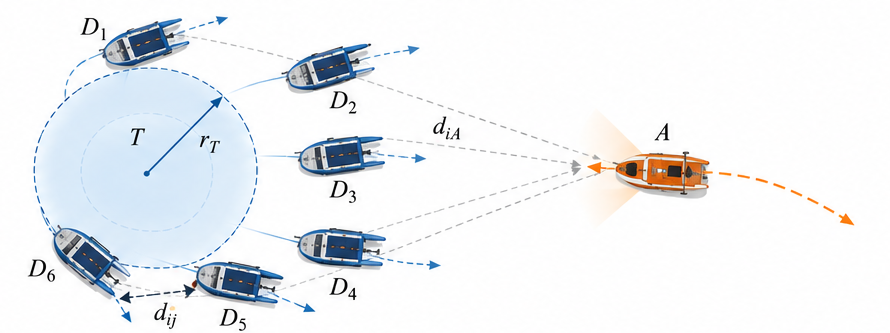
\includegraphics[width=5.4in]{figures/fig1_task.png}
\caption{六艇协同目标防御示意。蓝色艇为防御艇，橙色艇为攻击艇，圆形区域为受保护水域。虚线给出艇间及艇与攻击者之间的相对几何。}
\label{fig:1}
\end{figure}


捕获、艇间碰撞与物理突破事件分别由\(\min_i d_{iA}\le r_{\mathrm{cap}}\)、\(\min_{i<j}d_{ij}\le r_{\mathrm{col}}\)及\(\boldsymbol p_A\in\mathcal T\)确定。实验任务同时采用径向失守判据，当攻击艇到保护区中心的距离小于全部防御艇的径向距离时进入失守终止状态。相应事件集合为

\[
\begin{aligned}
\mathcal C&=\{x\mid\min_i d_{iA}\le r_{\mathrm{cap}}\},\\
\mathcal F_{\mathrm{col}}&=\{x\mid\min_{i<j}d_{ij}\le r_{\mathrm{col}}\},\\
\mathcal F_{\mathrm{rad}}&=\{x\mid\|\boldsymbol p_A\|<\min_i\|\boldsymbol p_i\|\}.
\end{aligned}
\tag{3}
\]

每个控制时刻按物理突破或径向失守、艇间碰撞、捕获和时间终止的顺序判定任务结局。任务在此前未进入失败状态的条件下完成捕获，或持续至规定时限\(T\)，记为防御成功。以\(Y\in\{0,1\}\)表示终局结果，协同控制目标写为

\[
\pi^\star\in\arg\max_\pi
\mathbb E_{x_0,\omega,\pi_A}[Y\mid\pi],
\qquad
\boldsymbol u_i(t)\in[u_D^{\min},u_D^{\max}]^2.
\tag{4}
\]

\(x_0\)为初始任务状态，\(\omega\)为环境与观测中的随机条件，\(\pi_A\)为攻击策略。控制器利用当前艇位、速度、相对几何及源控制指令形成联合决策，攻击者未来动作由实际对抗策略产生。各艇的当前信息汇集至联合融合计算过程，所得控制分量由各防御艇分别执行。数值评价将径向失守与终止前发生的物理突破分别记录。

\section{3
候选交互联合融合方法}\label{ux5019ux9009ux4ea4ux4e92ux8054ux5408ux878dux5408ux65b9ux6cd5}

\subsection{3.1
通道级融合与团队控制配置}\label{ux901aux9053ux7ea7ux878dux5408ux4e0eux56e2ux961fux63a7ux5236ux914dux7f6e}

CIV-RL以艇队的规则控制和学习控制组成为决策对象。设防御艇\(i\)的学习指令与规则指令分别为\(\boldsymbol u_i^L(x)\)和\(\boldsymbol u_i^B(x)\)，双通道融合变量为\(\boldsymbol g_i=[g_{i,1},g_{i,2}]^{\mathsf T}\in[0,1]^2\)，对应的推进器指令为

\[
\boldsymbol u_i(x,\boldsymbol g_i)=
\boldsymbol g_i\odot\boldsymbol u_i^L(x)
+(\boldsymbol 1-\boldsymbol g_i)\odot\boldsymbol u_i^B(x).
\tag{5}
\]

其中，\(\odot\)表示逐元素乘积。两侧推进器分别调节源控制的参与程度，整队融合配置记为\(\boldsymbol G=(\boldsymbol g_1,\ldots,\boldsymbol g_n)\)。两类源指令满足相同推力约束时，式（5）保持每个通道的输入有界性，并有

\[
\frac{\partial u_{i,a}}{\partial g_{i,a}}=u_{i,a}^{L}-u_{i,a}^{B},
\qquad
u_{i,a}\in\operatorname{co}\{u_{i,a}^{L},u_{i,a}^{B}\}.
\tag{6}
\]

融合变化的控制效应由源指令差异与融合系数共同确定。CI以各艇候选反馈响应为依据，将局部组成先验与艇对运动关系纳入统一配置评价，并构造参考策略\(\pi_0\)及其邻近联合方案。CV学习这些方案在后续闭环中的团队任务价值，在相同候选空间内确定是否采用替代配置。CI在各推进控制周期更新参考控制，CV在规定决策时刻选择有限作用区间内的融合方案，二者共同形成图2所示的控制与学习结构。

\begin{figure}[htbp]
\centering
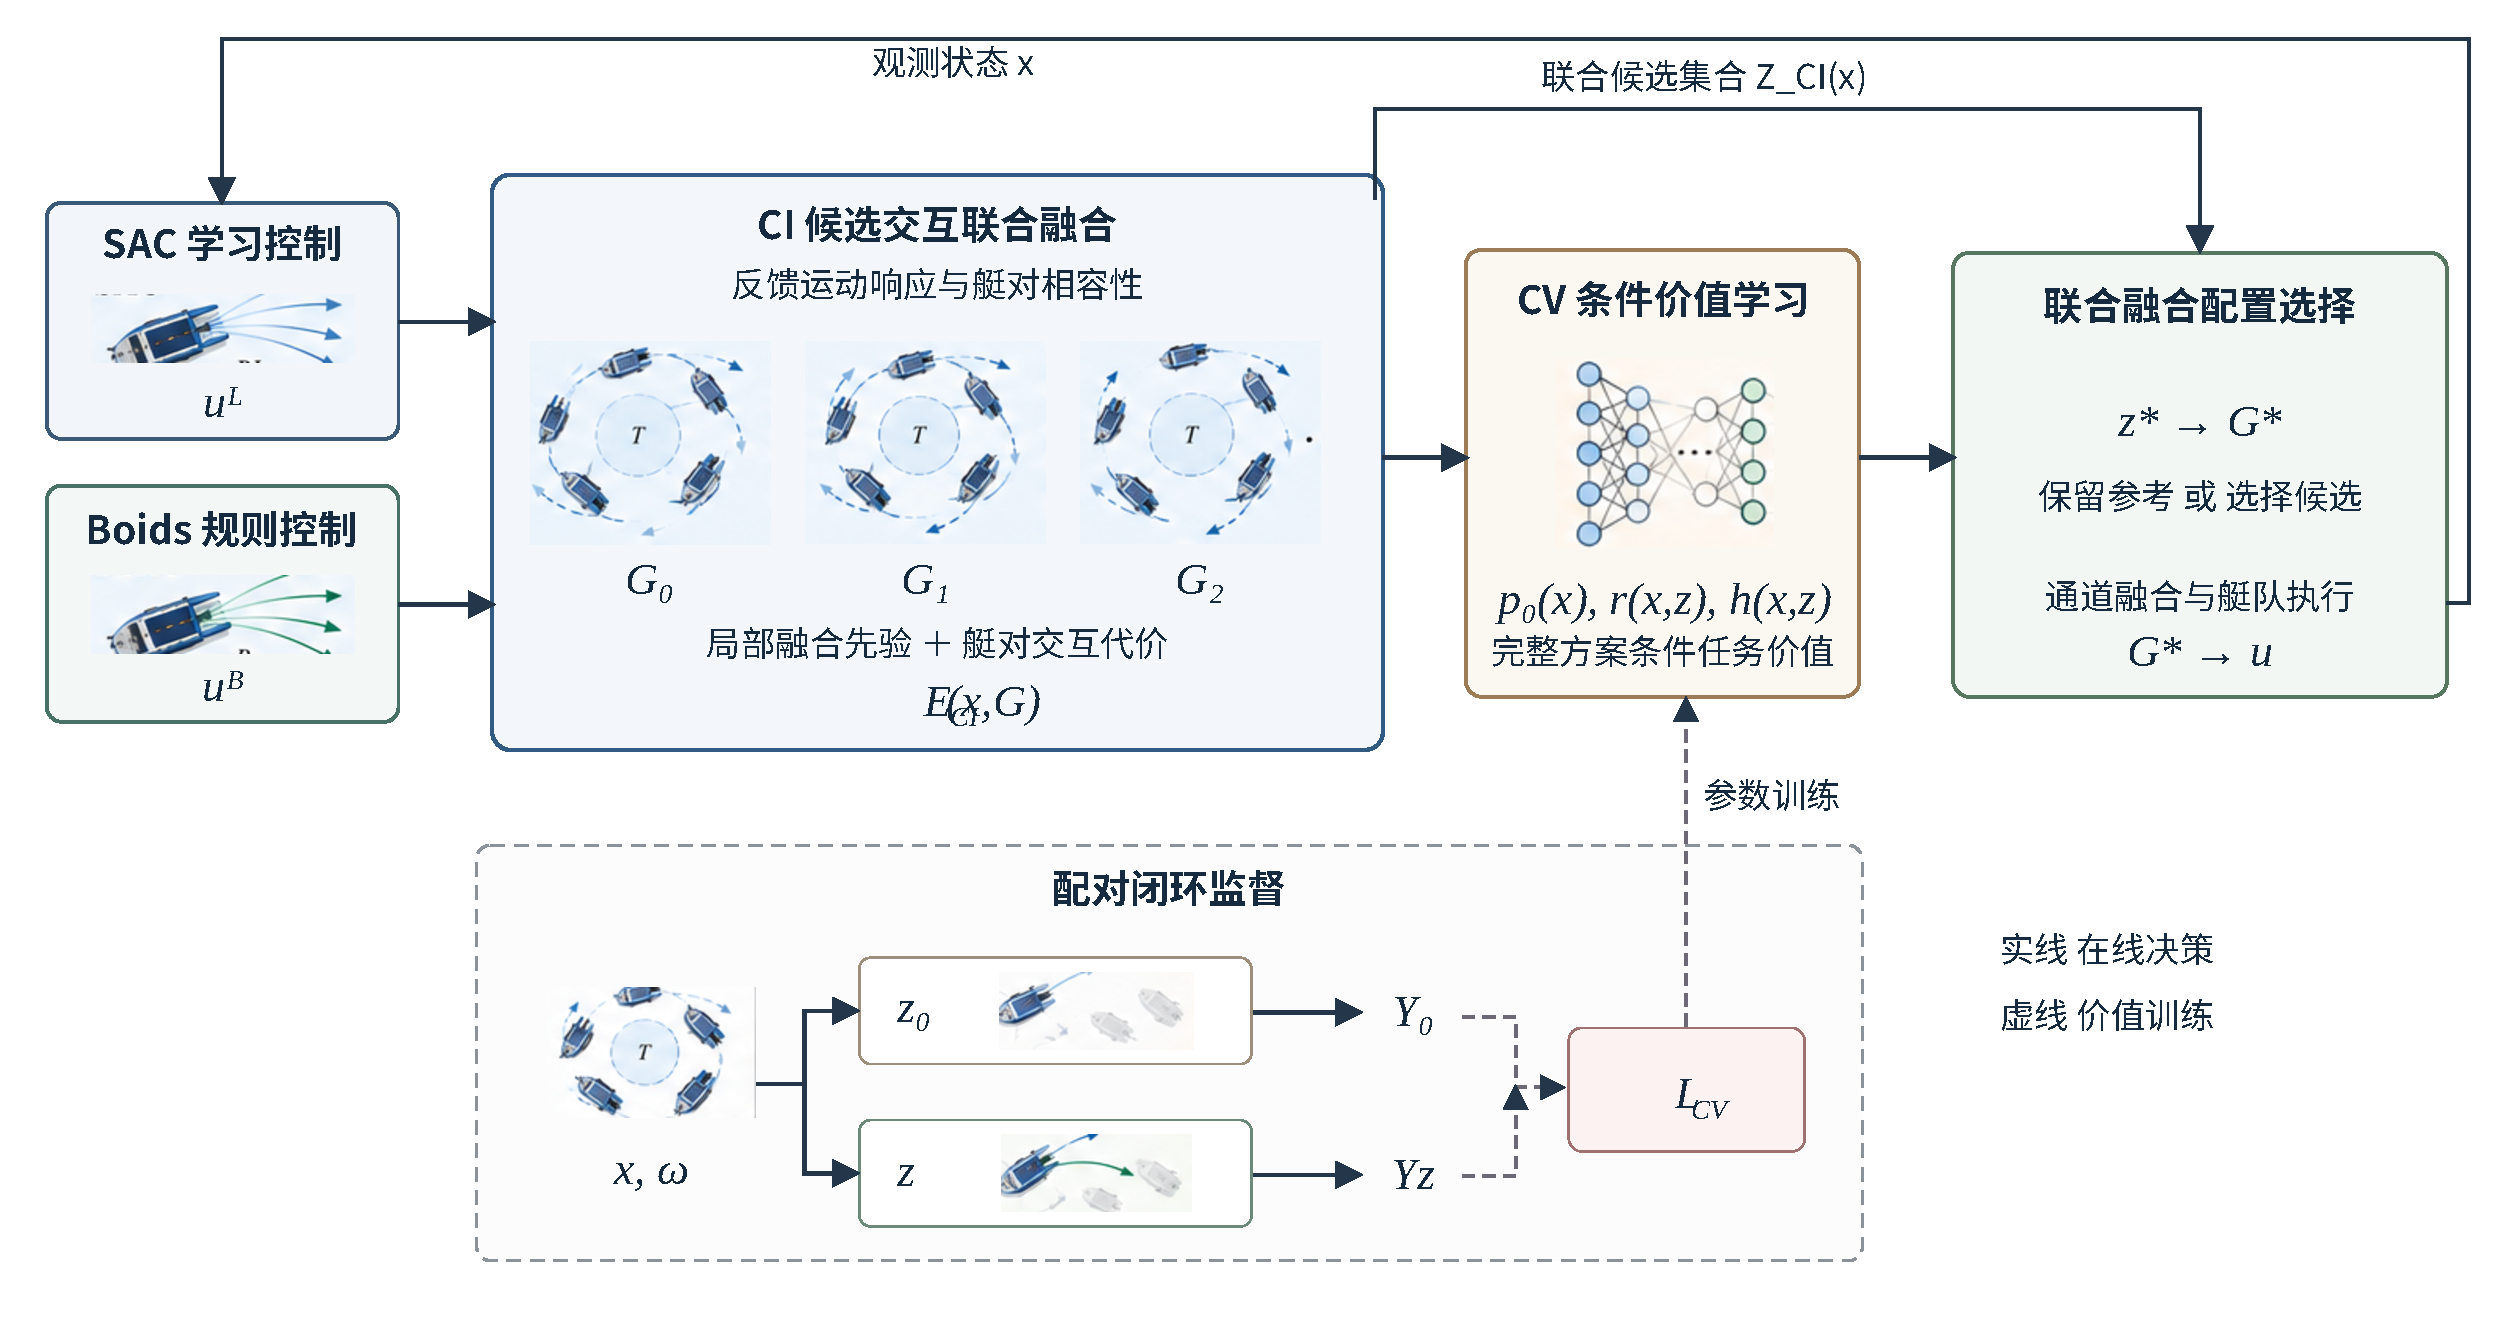
\includegraphics[width=6.35in]{figures/fig2_architecture.pdf}
\caption{CIV-RL的联合融合与价值学习结构。CI建立参考配置和联合候选，CV在同一方案空间内估计任务价值。实线表示在线信息流，虚线表示配对闭环监督与价值参数训练。}
\label{fig:2}
\end{figure}


\subsection{3.2
状态表示与源控制策略}\label{ux72b6ux6001ux8868ux793aux4e0eux6e90ux63a7ux5236ux7b56ux7565}

学习控制源采用参数共享的SAC策略{[}27{]}。局部观测由攻击艇与保护区域的相对方位和距离、队友相对状态以及Boids群体特征组成。队友观测经共享映射与均值聚合形成定长表示{[}12{]}，并与本艇和任务特征共同输入动作网络。若\(\mathcal N_i\)为防御艇\(i\)的队友集合，\(o_{ij}\)为相对观测，则状态编码为

\[
\boldsymbol e_i^D=\frac{1}{|\mathcal N_i|}
\sum_{j\in\mathcal N_i}f_D(o_{ij}),
\qquad
\boldsymbol h_i=f_s(o_i^{AT},\boldsymbol e_i^D,o_i^B).
\tag{7}
\]

\(o_i^{AT}\)表示攻击者和保护区域特征，\(o_i^B\)表示群体规则特征。动作网络输出学习指令，局部融合映射结合网络隐藏特征及两类源指令生成状态相关的组成偏好。该源策略采用文献{[}21{]}的自适应融合训练形式，动作生成器与局部融合映射通过任务回报共同预训练。冻结的源参数为后续CI和CV提供一致的控制候选。

SAC采用熵正则化目标

\[
J_{\mathrm{src}}(\psi)=
\mathbb E\left[
\sum_{t=0}^{T}\gamma^t
\bigl(r_t+\alpha\mathcal H(\pi_\psi(\cdot\mid o_t))\bigr)
\right],
\tag{8}
\]

其中，\(\gamma\)为折扣因子，\(\alpha\)为熵温度参数。各同构防御艇共享策略参数，其交互样本共同参与源策略训练。局部融合输出经有界映射形成候选中心\(\bar g_i(x)\)，并在两侧推进器中使用相同中心。

Boids控制由分离、对齐、聚合与目标吸引四类虚拟作用组成{[}7,21{]}

\[
\boldsymbol F_i=
\boldsymbol F_i^{\mathrm{sep}}
+\boldsymbol F_i^{\mathrm{ali}}
+\boldsymbol F_i^{\mathrm{coh}}
+\boldsymbol F_i^{\mathrm{att}}.
\tag{9}
\]

分离作用根据艇间相对位置产生排斥，对齐作用协调速度方向，聚合作用维持群体空间联系，目标吸引作用引导艇队接近攻击者。合力经艇体坐标变换及推进器映射得到规则指令\(\boldsymbol u_i^B\)。学习动作、规则动作与局部融合偏好共同规定单艇候选，候选之间的团队相容性由CI的联合模型评价。

\subsection{3.3
候选运动响应与交互配置}\label{ux5019ux9009ux8fd0ux52a8ux54cdux5e94ux4e0eux4ea4ux4e92ux914dux7f6e}

每艘防御艇的候选集合由规则端点、学习端点和局部融合中心构成。记\(\mathcal G_i(x)=\{\boldsymbol g_i^1,\ldots,\boldsymbol g_i^{K_i}\}\)，通道组合取自\(\{0,\bar g_i,1\}^2\)，重合的系数组合合并为同一候选。局部先验代价表示候选相对于源融合建议的偏离

\[
\phi_i(k;x)=\frac{1}{2}\sum_{a=1}^{2}
\left(\frac{g_{i,a}^{k}-\bar g_i(x)}{\sigma_g}\right)^2.
\tag{10}
\]

\(\sigma_g\)给出偏离尺度。局部先验在当前候选之间保持源策略形成的状态偏好，候选的联合评价进一步包含其与其他艇运动响应之间的关系。

候选反馈预测以当前观测状态为起点，在时域\(H\)内保持候选融合系数，并根据预测状态重新计算学习与规则指令。以\(\widehat F\)表示名义状态转移，防御艇\(i\)执行候选\(k\)时的预测递推为

\[
\widehat x_{\ell+1}^{i,k}
=\widehat F\bigl(\widehat x_\ell^{i,k},
\boldsymbol u_i(\widehat x_\ell^{i,k},\boldsymbol g_i^k)\bigr),
\qquad \widehat x_0^{i,k}=x.
\tag{11}
\]

相邻艇的名义运动用于构造预测观测。各候选分别形成位置序列\(\widehat{\boldsymbol p}_i^k(t)\)，候选系数保持时，两类源指令仍随状态反馈变化。对艇\(i\)和\(j\)的候选组合\((k,\ell)\)，定义最小预测间距及艇对交互势

\[
\begin{aligned}
d_{ij}^{k\ell}(x)&=\min_{t\in[0,H]}
\|\widehat{\boldsymbol p}_i^k(t)-\widehat{\boldsymbol p}_j^\ell(t)\|,\\
\psi_{ij}(k,\ell;x)&=[r_s-d_{ij}^{k\ell}(x)]_+^2.
\end{aligned}
\tag{12}
\]

\(r_s\)为候选接近评价距离，\([a]_+=\max(a,0)\)。该交互势依赖双方候选，同一局部组成在不同队友配置下具有不同的运动代价。以候选索引向量\(\boldsymbol k=(k_1,\ldots,k_n)\)表示整队配置，联合能量定义为

\[
E_{\mathrm{CI}}(x,\boldsymbol k)=
\sum_{i=1}^{n}\phi_i(k_i;x)
+\lambda\sum_{i<j}\psi_{ij}(k_i,k_j;x).
\tag{13}
\]

\(\lambda\)控制艇对交互的作用。参考配置通过最小化式（13）获得，其候选索引记为\(\boldsymbol k_0\)，融合组成记为\(\boldsymbol G_0(x)\)。在保持其他艇选择不变时，艇\(i\)由\(k_i\)变为\(k_i'\)所引起的能量变化为

\[
\delta E_i=
\phi_i(k_i';x)-\phi_i(k_i;x)
+\lambda\sum_{j\ne i}
\bigl[\psi_{ij}(k_i',k_j;x)-\psi_{ij}(k_i,k_j;x)\bigr].
\tag{14}
\]

式（14）使局部融合的评价显式依赖于队友正在选择的控制组成。联合求解采用束搜索与坐标细化，在组合空间内同时考虑个体偏离和艇对运动代价。参考配置、保留的联合搜索结果以及参考配置的单艇邻域共同形成备选池，候选按联合能量排序，并在给定代价容差内选取

\[
\mathcal C(x)=\{\boldsymbol G_0(x)\}\cup
\left\{\boldsymbol G\in\mathcal P(x)\ 
\middle|\ 
E_{\mathrm{CI}}(x,\boldsymbol G)
\le E_{\mathrm{CI}}(x,\boldsymbol G_0)+n\rho\right\}.
\tag{15}
\]

其中，\(\mathcal P(x)\)为联合候选池，\(\rho\)为单位艇数的能量容差，候选数量受统一规模限制。CI由此同时确定参考控制和供条件价值评价的完整方案空间。图3将艇对候选运动与配对闭环任务后果并列表示，两类评价作用于同一融合配置。

\begin{figure}[htbp]
\centering
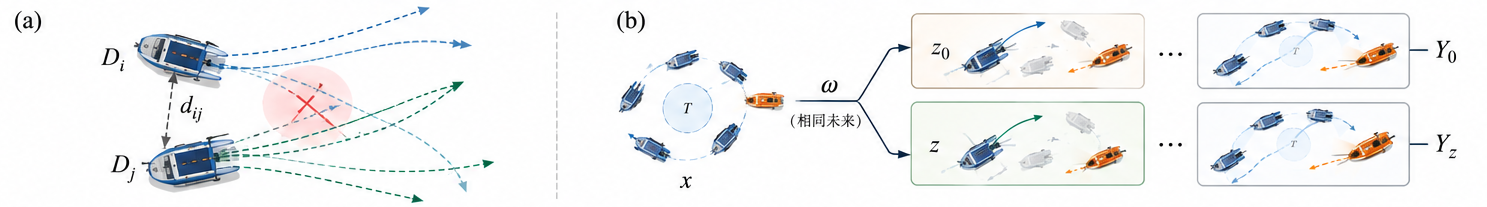
\includegraphics[width=6.35in]{figures/fig3_mechanism.png}
\caption{候选交互与配对闭环关系。（a）不同融合候选的运动相容性。（b）同一根状态与共同随机未来下的参考方案和替代方案，终局结果分别为$Y_0$与$Y_z$。}
\label{fig:3}
\end{figure}


\subsection{3.4
配对闭环条件价值}\label{ux914dux5bf9ux95edux73afux6761ux4ef6ux4ef7ux503c}

完整融合方案记为\(z=(\boldsymbol G,d,\tau)\)，分别给出联合组成、执行延迟与作用时长。参考方案\(z_0\)持续采用CI参考策略\(\pi_0\)。候选方案在规定区间内保持选定融合系数，学习和规则指令根据各分支的实时状态更新，在区间之前和结束之后执行相同的参考策略。以\(t_d\)表示方案决策时刻，其系数过程为

\[
\boldsymbol g_i(t;z)=
\begin{cases}
\boldsymbol g_i^z,&t_d+d\le t<t_d+d+\tau,\\
\boldsymbol g_i^0(x_t),&\text{其他时刻}.
\end{cases}
\tag{16}
\]

候选\(\boldsymbol G\)来自式（15）的联合配置，时序参数与配置共同确定完整闭环控制过程。在共同根状态\(x\)和随机未来\(\omega\)下，终局结果及条件价值定义为

\[
Y(x,z,\omega)=\mathbb I\{\text{闭环续行防御成功}\},
\qquad
V^{\pi_0}(x,z)=\mathbb E_\omega[Y(x,z,\omega)].
\tag{17}
\]

配对分支具有相同的根状态、源策略参数和外部随机条件，各自在到达状态上重新生成反馈控制。参考配置的单艇邻域形成局部组成比较，联合搜索得到的多艇配置则以完整方案接受评价。对任意两个可比较方案\(z\)与\(z'\)，经验条件差值为

\[
\widehat\Delta(x;z,z')=
\frac{1}{R_x}\sum_{q=1}^{R_x}
\bigl[Y(x,z',\omega_q)-Y(x,z,\omega_q)\bigr].
\tag{18}
\]

\(R_x\)为该根状态下的配对未来数。相同未来条件使两种配置的结果围绕同一任务扰动比较，训练保留成功与失败终局以及对应的参考结果。完整方案价值由共享函数表示，任意局部或联合变化的预测差均由同一价值基准得到

\[
\Delta_\theta(x;z,z')=V_\theta(x,z')-V_\theta(x,z).
\tag{19}
\]

记\(Y_0=Y(x,z_0,\omega)\)、\(Y_z=Y(x,z,\omega)\)。条件模型分别表示参考成功概率、参考失败条件下的候选成功概率以及参考成功条件下的候选失败概率

\[
\begin{aligned}
p_{0,\theta}(x)&=\Pr(Y_0=1\mid x),\\
r_\theta(x,z)&=\Pr(Y_z=1\mid Y_0=0,x),\\
h_\theta(x,z)&=\Pr(Y_z=0\mid Y_0=1,x).
\end{aligned}
\tag{20}
\]

完整候选价值和相对于参考的净收益写为

\[
\begin{aligned}
V_\theta(x,z)&=[1-p_{0,\theta}(x)]r_\theta(x,z)
+p_{0,\theta}(x)[1-h_\theta(x,z)],\\
\Delta_\theta(x;z_0,z)&=[1-p_{0,\theta}(x)]r_\theta(x,z)
-p_{0,\theta}(x)h_\theta(x,z),\\
V_\theta(x,z_0)&=p_{0,\theta}(x).
\end{aligned}
\tag{21}
\]

该参数化将候选的团队任务价值与参考策略的成功水平联系起来。候选结果在事实失败和事实成功条件下分别接受监督，经式（21）形成统一价值，并通过式（19）参与完整配置间的比较。CI的运动交互评价规定候选结构，CV的条件任务评价刻画这些配置在后续防御中的收益。

\subsection{3.5
关系表示与条件监督训练}\label{ux5173ux7cfbux8868ux793aux4e0eux6761ux4ef6ux76d1ux7763ux8badux7ec3}

条件价值网络以完整团队配置为输入。艇节点特征包含当前相对位置、速度与艏向、源学习指令、参考融合系数、候选融合系数、系数差以及候选预测终点。艇对特征由相对位置、相对速度、候选终点差和预测交互势组成，方案级特征包含任务时间、联合代价统计和作用区间。节点与艇对特征首先进入共享关系映射，艇间消息经注意力加权后更新节点表示

\[
\begin{aligned}
\boldsymbol h_i&=f_n(\boldsymbol\xi_i),\\
a_{ij}&=
\frac{\exp f_a(\boldsymbol h_i,\boldsymbol h_j,\boldsymbol\rho_{ij})}
{\sum_{k\ne i}\exp f_a(\boldsymbol h_i,\boldsymbol h_k,\boldsymbol\rho_{ik})},\\
\boldsymbol h_i^+&=f_u\left(\boldsymbol h_i,
\sum_{j\ne i}a_{ij}f_m(\boldsymbol h_i,\boldsymbol h_j,\boldsymbol\rho_{ij})\right).
\end{aligned}
\tag{22}
\]

对当前有效艇集合采用均值和最大值聚合，得到方案表示\(\boldsymbol H_z\)。读出层共同使用参考表示、候选表示及其差异，并结合方案级特征\(\boldsymbol e_z\)输出条件概率参数

\[
\begin{aligned}
\boldsymbol H_z&=
\left[\operatorname{Mean}_i\boldsymbol h_i^+,
\operatorname{Max}_i\boldsymbol h_i^+\right],\\
\boldsymbol l_\theta(x,z)&=
 f_o(\boldsymbol H_{z_0},\boldsymbol H_z-\boldsymbol H_{z_0},
 \boldsymbol H_z,\boldsymbol e_{z_0},\boldsymbol e_z).
\end{aligned}
\tag{23}
\]

参考成功概率由参考方案的输出获得，条件成功与失败概率由候选输出经Sigmoid映射得到。共享节点映射及艇队聚合适用于不同数量的防御艇，融合系数与实际艇的对应关系贯穿候选编码和控制执行。输入特征的标准化统计由训练数据确定，在验证和部署过程中保持固定。

设\(\ell(p,y)=-y\log p-(1-y)\log(1-p)\)，条件概率学习采用参考结果和条件结果的二元交叉熵。以训练数据分布\(\mathcal D\)及其事实条件子集表示相应期望，目标写为

\[
\begin{aligned}
\mathcal L_{\mathrm{prob}}={}&
\mathbb E_{\mathcal D}\ell(p_{0,\theta},Y_0)\\
&+\frac12\mathbb E_{\mathcal D\mid Y_0=0}\ell(r_\theta,Y_z)
+\frac12\mathbb E_{\mathcal D\mid Y_0=1}\ell(h_\theta,1-Y_z).
\end{aligned}
\tag{24}
\]

各条件项按有效候选及相应事实事件的样本质量归一化。参考标签由同一根状态下的未来结果形成，候选条件标签保留对应的事实分组。训练对根状态进行自助重采样，并按实际采样概率校正根状态的目标权重。

配对收益监督以各根状态下的平均终局差\(\bar\delta_{xz}=R_x^{-1}\sum_q(Y_z^{(q)}-Y_0^{(q)})\)为目标。参考概率在该损失路径中采用梯度截断，定义

\[
\widetilde\Delta_\theta(x,z)=
[1-\operatorname{sg}(p_{0,\theta}(x))]r_\theta(x,z)
-\operatorname{sg}(p_{0,\theta}(x))h_\theta(x,z).
\tag{25}
\]

配对项及完整学习目标为

\[
\begin{aligned}
\mathcal L_\Delta&=
\frac{\sum_{x,z\ne z_0}w_{xz}
[\widetilde\Delta_\theta(x,z)-\bar\delta_{xz}]^2}
{\sum_{x,z\ne z_0}w_{xz}},\\
w_{xz}&=\iota_xm_{xz}(1+3|\bar\delta_{xz}|),\\
\mathcal L_{\mathrm{CV}}&=\mathcal L_{\mathrm{prob}}+\lambda_\Delta\mathcal L_\Delta.
\end{aligned}
\tag{26}
\]

其中，\(m_{xz}\)为候选有效掩码，\(\iota_x\)为根状态采样校正权重。条件似然拟合参考成功和候选后果，配对项直接约束相对于参考的收益估计。网络参数由式（26）更新，源策略与CI的候选生成参数在该阶段冻结。不同模型成员对根状态采用独立自助采样，部署价值由成员输出平均得到。

\subsection{3.6
条件价值引导的联合选择}\label{ux6761ux4ef6ux4ef7ux503cux5f15ux5bfcux7684ux8054ux5408ux9009ux62e9}

CI提供的完整候选方案经统一的可执行定义进入CV评价。参考方案始终保留在候选集中，其相对收益固定为零。记模型成员的平均预测收益为\(\bar\Delta_\theta(x,z)\)，接受阈值为\(\varepsilon\)，最终方案按照

\[
S_\theta(x,z)=
\begin{cases}
0,&z=z_0,\\
\bar\Delta_\theta(x,z)-\varepsilon,&z\ne z_0,
\end{cases}
\qquad
z^\star\in\arg\max_{z\in\mathcal Z_{\mathrm{CI}}(x)}S_\theta(x,z)
\tag{27}
\]

确定。并列最高分为零时选择参考方案。候选的运动交互通过式（13）和式（15）进入方案空间，闭环任务信息通过式（21）和式（27）进入最终排序。选定方案按照式（16）的融合系数过程作用于当前源指令，形成

\[
\boldsymbol u_i(t)=
\boldsymbol g_i(t;z^\star)\odot\boldsymbol u_i^L(x_t)
+[\boldsymbol1-\boldsymbol g_i(t;z^\star)]\odot\boldsymbol u_i^B(x_t).
\tag{28}
\]

在方案作用区间内，艇队持续获得状态反馈，两类源动作随状态重新计算；区间结束后由CI恢复参考联合选择。配对数据生成与在线运行使用相同的方案时序、融合映射和后续控制关系。由此，候选交互建模、条件价值学习和最终推进控制共同作用于统一的团队融合变量。

\subsection{3.7
奖励与训练过程}\label{ux5956ux52b1ux4e0eux8badux7ec3ux8fc7ux7a0b}

源策略训练采用任务奖励、队形奖励与碰撞惩罚的组合{[}21{]}

\[
r_i=r_i^{\mathrm{task}}+r_i^{\mathrm{form}}+r_i^{\mathrm{col}}.
\tag{29}
\]

任务项根据防御失败、目标捕获及近邻协助给出反馈。完成捕获的防御艇获得捕获奖励，位于捕获邻域内的协助艇获得协作奖励。队形项利用防御艇至攻击艇的单位方向和保护区至攻击艇的方向构造拦截分布。令\(\widehat{\boldsymbol d}_{iA}=(\boldsymbol p_A-\boldsymbol p_i)/\|\boldsymbol p_A-\boldsymbol p_i\|\)、\(\boldsymbol d_{DA}=\sum_i\widehat{\boldsymbol d}_{iA}\)、\(\widehat{\boldsymbol d}_{TA}=\boldsymbol p_A/\|\boldsymbol p_A\|\)，则

\[
r_i^{\mathrm{form}}=
0.5\widehat{\boldsymbol d}_{TA}^{\mathsf T}
\frac{\boldsymbol d_{DA}}{\|\boldsymbol d_{DA}\|}
-\frac{\|\boldsymbol d_{DA}\|}{n}.
\tag{30}
\]

零范数时相应方向项取零，碰撞惩罚由艇间距离阈值触发。任务与碰撞反馈共同确定源控制的优化方向，CV则直接以团队终局结果学习融合方案的条件任务价值。两类反馈分别作用于源动作生成和团队组成评价。

源策略采用攻击者机动性课程{[}28{]}，每回合从\(\mathcal U(\bar L_{\mathrm{agi}}-0.5,\bar L_{\mathrm{agi}}+0.5)\)采样攻击者机动系数，平均机动性随训练推进逐步提高。完成源策略学习后，固定控制来源，构建CI联合候选并采集配对闭环后果，再训练条件价值网络。模型选择依据开发验证任务，冻结后的完整控制器用于最终任务评价。

\section{4 实验与分析}\label{ux5b9eux9a8cux4e0eux5206ux6790}

\subsection{4.1 实验设置}\label{ux5b9eux9a8cux8bbeux7f6e}

数值评价采用六艘防御艇对单艘攻击艇的区域防御任务。保护区域半径为15
m，捕获距离与艇间碰撞距离均为5 m，任务时限为80 s。动力学积分周期为0.05
s，推进器控制周期为0.2 s，单推进器推力范围为\([-500,1000]\)
N。攻击艇采用根据目标吸引和防御艇排斥形成的人工势场策略，主评价覆盖\(L_{\mathrm{agi}}=2.0\)和2.5。初始位置、航向及随机未来按共同任务协议生成，各方法在相同任务上配对评价。

CI预测时域为3.2 s，预测步长为0.1 s，学习与规则指令按0.2
s更新。联合配置使用局部先验尺度0.4和交互权重32，候选束宽为128。价值评价保留至多6个联合配置，以单位艇数0.5的代价容差筛选备选方案。CV在第20个控制时刻进行一次方案选择，候选作用时长为5或20个控制周期，执行延迟为零。候选接受阈值在开发任务中确定为0.075，最终评价沿用该配置。

源学习策略在六艇条件下完成\(10^6\)步环境交互，并通过训练评价确定检查点。条件价值训练使用772个根状态，验证使用206个根状态，场景及其配对未来保持在同一数据划分。三个关系网络成员采用独立根状态自助采样，每个成员具有96
420个可训练参数，隐藏维数为64。训练上限为每成员4
500次更新，条件价值的选定检查点为每成员1
500次更新，普通价值对照选用每成员4
500次更新。两者共用源控制、关系网络、候选定义、训练样本和最大更新预算。主要参数见表1。

\Needspace{6\baselineskip}
\begin{center}\small 表1　任务与方法参数\end{center}

\begingroup\small
\begin{longtable}[]{@{}lll@{}}
\toprule\noalign{}
参数 & 符号 & 设置 \\
\midrule\noalign{}
\endhead
\bottomrule\noalign{}
\endlastfoot
主任务艇数 & \(n\) & 6 \\
任务时限 & \(T\) & 80 s \\
控制周期 & \(\Delta t\) & 0.2 s \\
动力学积分周期 & \(\Delta t_{\mathrm{int}}\) & 0.05 s \\
保护区域半径 & \(r_T\) & 15 m \\
数值捕获与碰撞阈值 & \(r_{\mathrm{cap}},r_{\mathrm{col}}\) & 5 m，5 m \\
CI预测时域 & \(H\) & 3.2 s \\
候选接近距离 & \(r_s\) & 7 m \\
局部先验尺度 & \(\sigma_g\) & 0.4 \\
交互权重 & \(\lambda\) & 32 \\
联合候选数上限 & \(K_G\) & 6 \\
单位艇数代价容差 & \(\rho\) & 0.5 \\
CV决策时刻 & \(t_d\) & 4 s \\
候选作用时长 & \(\tau\) & 1 s，4 s \\
候选执行延迟 & \(d\) & 0 s \\
接受阈值 & \(\varepsilon\) & 0.075 \\
训练与验证根状态 & & 772，206 \\
价值网络成员数 & & \(3\) \\
单成员可训练参数 & & \(96\,420\) \\
最大更新次数／成员 & & \(4\,500\) \\
选定CV更新次数／成员 & & \(1\,500\) \\
学习率 & & \(3\times10^{-4}\) \\
配对收益损失权重 & \(\lambda_\Delta\) & 2 \\
主评价任务数 & \(N\) & 200 \\
\end{longtable}
\endgroup

正式主评价包含200个独立任务，每种方法使用一个冻结的训练流程。任务成功比例报告Wilson
95\%置信区间，直接机制比较采用逐任务配对结果。记被比较方法与参考方法的结果为\(Y_e^\pi\)和\(Y_e^{\pi_b}\)，配对成功率差为

\[
\widehat\delta_{\mathrm{SR}}(\pi,\pi_b)=
\frac{1}{N}\sum_{e=1}^{N}(Y_e^\pi-Y_e^{\pi_b})
=\frac{N_{01}-N_{10}}{N},
\tag{31}
\]

其中，\(N_{01}\)为参考失败而被比较方法成功的任务数，\(N_{10}\)为参考成功而被比较方法失败的任务数。数值试验同时记录捕获、碰撞、径向失守、物理突破和任务时长。捕获时间以成功捕获回合为统计总体，两种策略共同捕获的任务另行计算配对时间差。源策略环境交互、配对闭环续行及价值网络更新分别计量，在线计算覆盖候选预测、联合求解与价值选择。独立完整训练的均值、标准差及运行间差值列于补充表S2，相应统计数值为［　］。

\subsection{4.2
高保真闭环防御}\label{ux9ad8ux4fddux771fux95edux73afux9632ux5fa1}

高保真试验在Gazebo
VRX水面环境中运行WAM-V防御艇与攻击艇，完整方法、仅CI和ARBoids采用相同初始位置、推力接口及控制周期。任务时限为80
s，保护区域半径为15 m，艇间碰撞阈值为5 m，捕获阈值为5.5
m。12组共同场景共形成36次有效闭环任务。图4展示其中一组场景的真实仿真画面与记录轨迹，防御艇从保护水域附近出发，通过不同推进和转向组合接近攻击者，在攻击者进入目标区域之前形成捕获。

\begin{figure}[htbp]
\centering
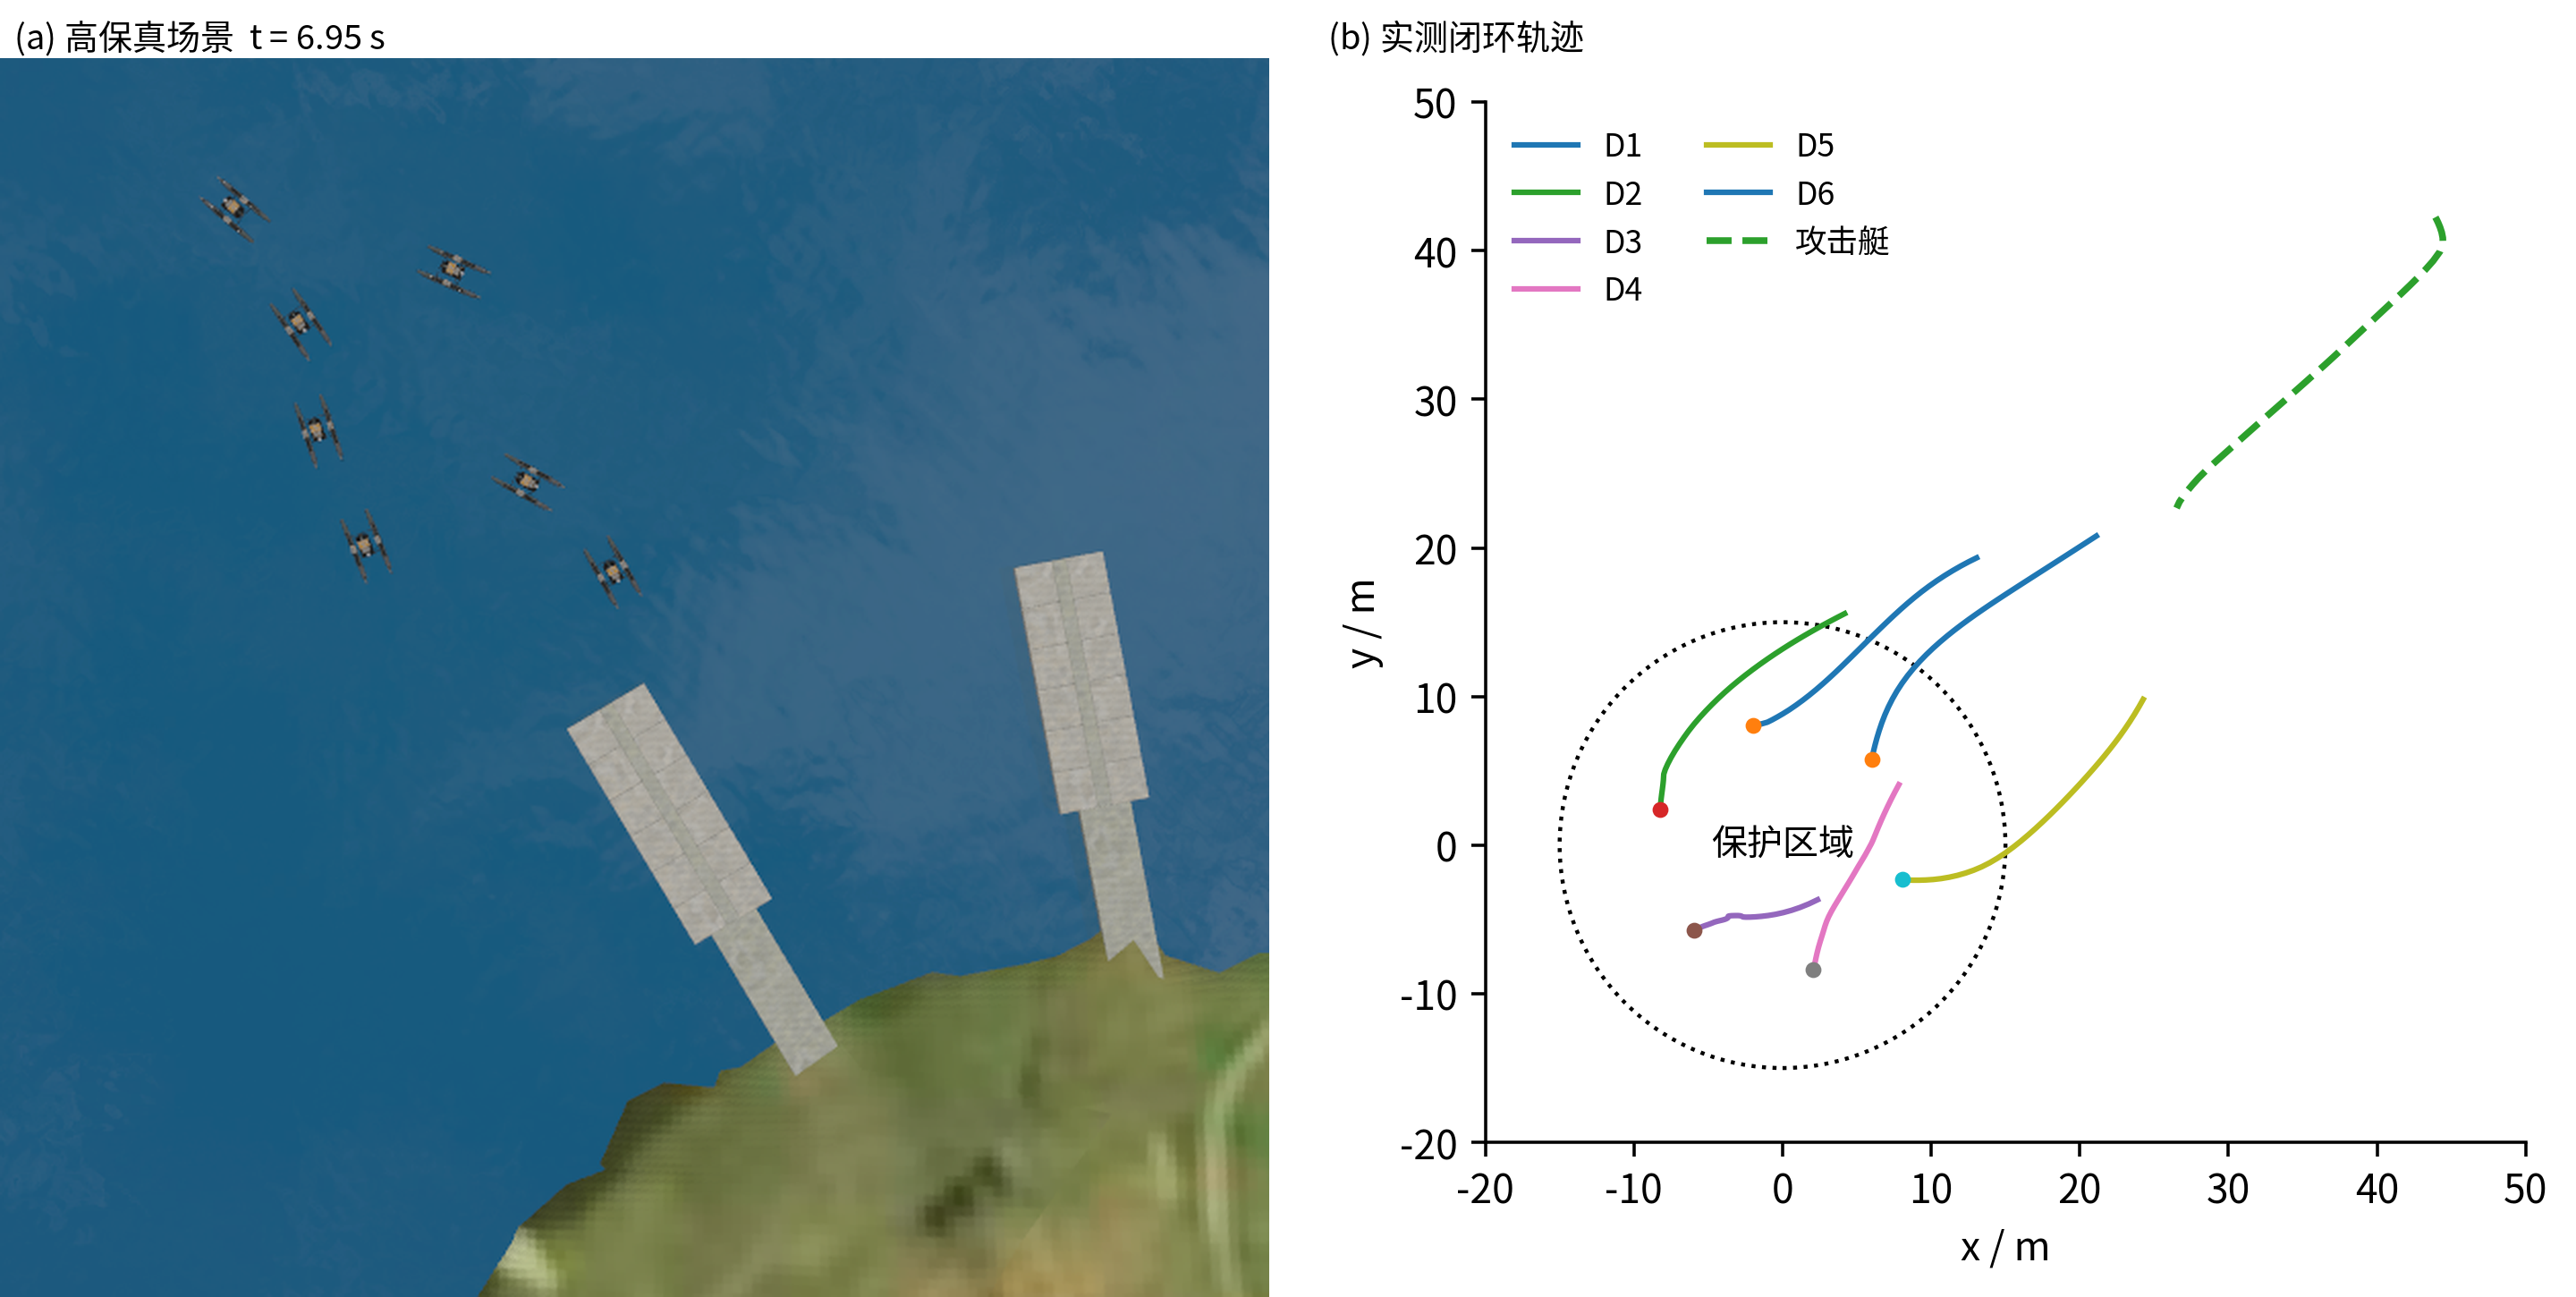
\includegraphics[width=6.35in]{figures/fig4_vrx.png}
\caption{真实VRX防御场景及对应轨迹。（a）规定场景序列中的首个场景，在6.95 s时的仿真画面。（b）同一任务的记录轨迹，攻击艇在7.85 s时被捕获。}
\label{fig:4}
\end{figure}


CIV-RL与仅CI均在12组场景中完成捕获，ARBoids完成11次捕获，另一次以艇间碰撞终止。相应成功捕获平均时间分别为8.88
s、8.80 s和7.85
s。完整方法的候选选择保持了CI所形成的联合拦截能力，艇队在全部配对场景中维持有效的运动分离。该组高保真结果与数值主评价中较低的艇间碰撞率相对应，表现出联合融合模型在不同动力学实现中的可执行性。

在线时延按每个有效控制周期记录。CIV-RL的平均决策时间为119.09
ms，95\%分位为169.61 ms；仅CI对应为118.25 ms和165.39
ms。两者的95\%分位均低于200
ms控制周期。CIV-RL有2.22\%的控制样本超过该周期，仅CI为2.62\%，完整记录见表2。条件价值评价在联合候选优化的基础上参与控制，其实际时延由候选预测、配置求解和网络评价共同构成。

\Needspace{6\baselineskip}
\begin{center}\small 表2　VRX配对任务与决策时延\end{center}

\begingroup\small
\begin{longtable}[]{@{}
  >{\raggedright\arraybackslash}p{(\columnwidth - 12\tabcolsep) * \real{0.1429}}
  >{\raggedright\arraybackslash}p{(\columnwidth - 12\tabcolsep) * \real{0.1429}}
  >{\raggedright\arraybackslash}p{(\columnwidth - 12\tabcolsep) * \real{0.1429}}
  >{\raggedright\arraybackslash}p{(\columnwidth - 12\tabcolsep) * \real{0.1429}}
  >{\raggedright\arraybackslash}p{(\columnwidth - 12\tabcolsep) * \real{0.1429}}
  >{\raggedright\arraybackslash}p{(\columnwidth - 12\tabcolsep) * \real{0.1429}}
  >{\raggedright\arraybackslash}p{(\columnwidth - 12\tabcolsep) * \real{0.1429}}@{}}
\toprule\noalign{}
\begin{minipage}[b]{\linewidth}\raggedright
方法
\end{minipage} & \begin{minipage}[b]{\linewidth}\raggedright
捕获数
\end{minipage} & \begin{minipage}[b]{\linewidth}\raggedright
碰撞数
\end{minipage} & \begin{minipage}[b]{\linewidth}\raggedright
平均捕获／s
\end{minipage} & \begin{minipage}[b]{\linewidth}\raggedright
平均时延／ms
\end{minipage} & \begin{minipage}[b]{\linewidth}\raggedright
95\%分位／ms
\end{minipage} & \begin{minipage}[b]{\linewidth}\raggedright
超期比例／\%
\end{minipage} \\
\midrule\noalign{}
\endhead
\bottomrule\noalign{}
\endlastfoot
CIV-RL & 12/12 & 0 & 8.88 & 119.09 & 169.61 & 2.22 \\
仅CI & 12/12 & 0 & 8.80 & 118.25 & 165.39 & 2.62 \\
ARBoids & 11/12 & 1 & 7.85 & 3.50 & 4.37 & 0.00 \\
\end{longtable}
\endgroup

\subsection{4.3
基线比较与机制分析}\label{ux57faux7ebfux6bd4ux8f83ux4e0eux673aux5236ux5206ux6790}

\subsubsection{4.3.1
整体性能与学习过程}\label{ux6574ux4f53ux6027ux80fdux4e0eux5b66ux4e60ux8fc7ux7a0b}

竞争性比较包含Boids、SAC、传统残差策略RP、自适应残差方法ARBoids和MAPPO{[}14,18,21,27{]}。Boids执行群体规则指令，SAC直接学习连续推进控制，RP叠加规则动作与学习残差，ARBoids通过状态相关权重形成源动作融合，MAPPO采用集中式价值训练与分布式策略执行。各学习基线在六艇任务中按照自身结构训练，环境交互预算为\(10^6\)步。所有方法接受相同的任务终止判据与正式评价场景。

完整方法设置两项核心消融。w/o
CI以局部融合评价形成候选组合，移除艇对交互和联合配置优化，条件价值模型依据该参考控制重新采集的数据训练。w/o
CV保留CI的候选预测、交互评价和联合求解，直接执行参考配置。w/o
CI的价值模型采用相同关系结构和每成员4
500次更新，其训练和验证根状态数分别为158和31。两项消融与五种已有算法共同构成表3的八项主比较。

\begin{figure}[htbp]
\centering
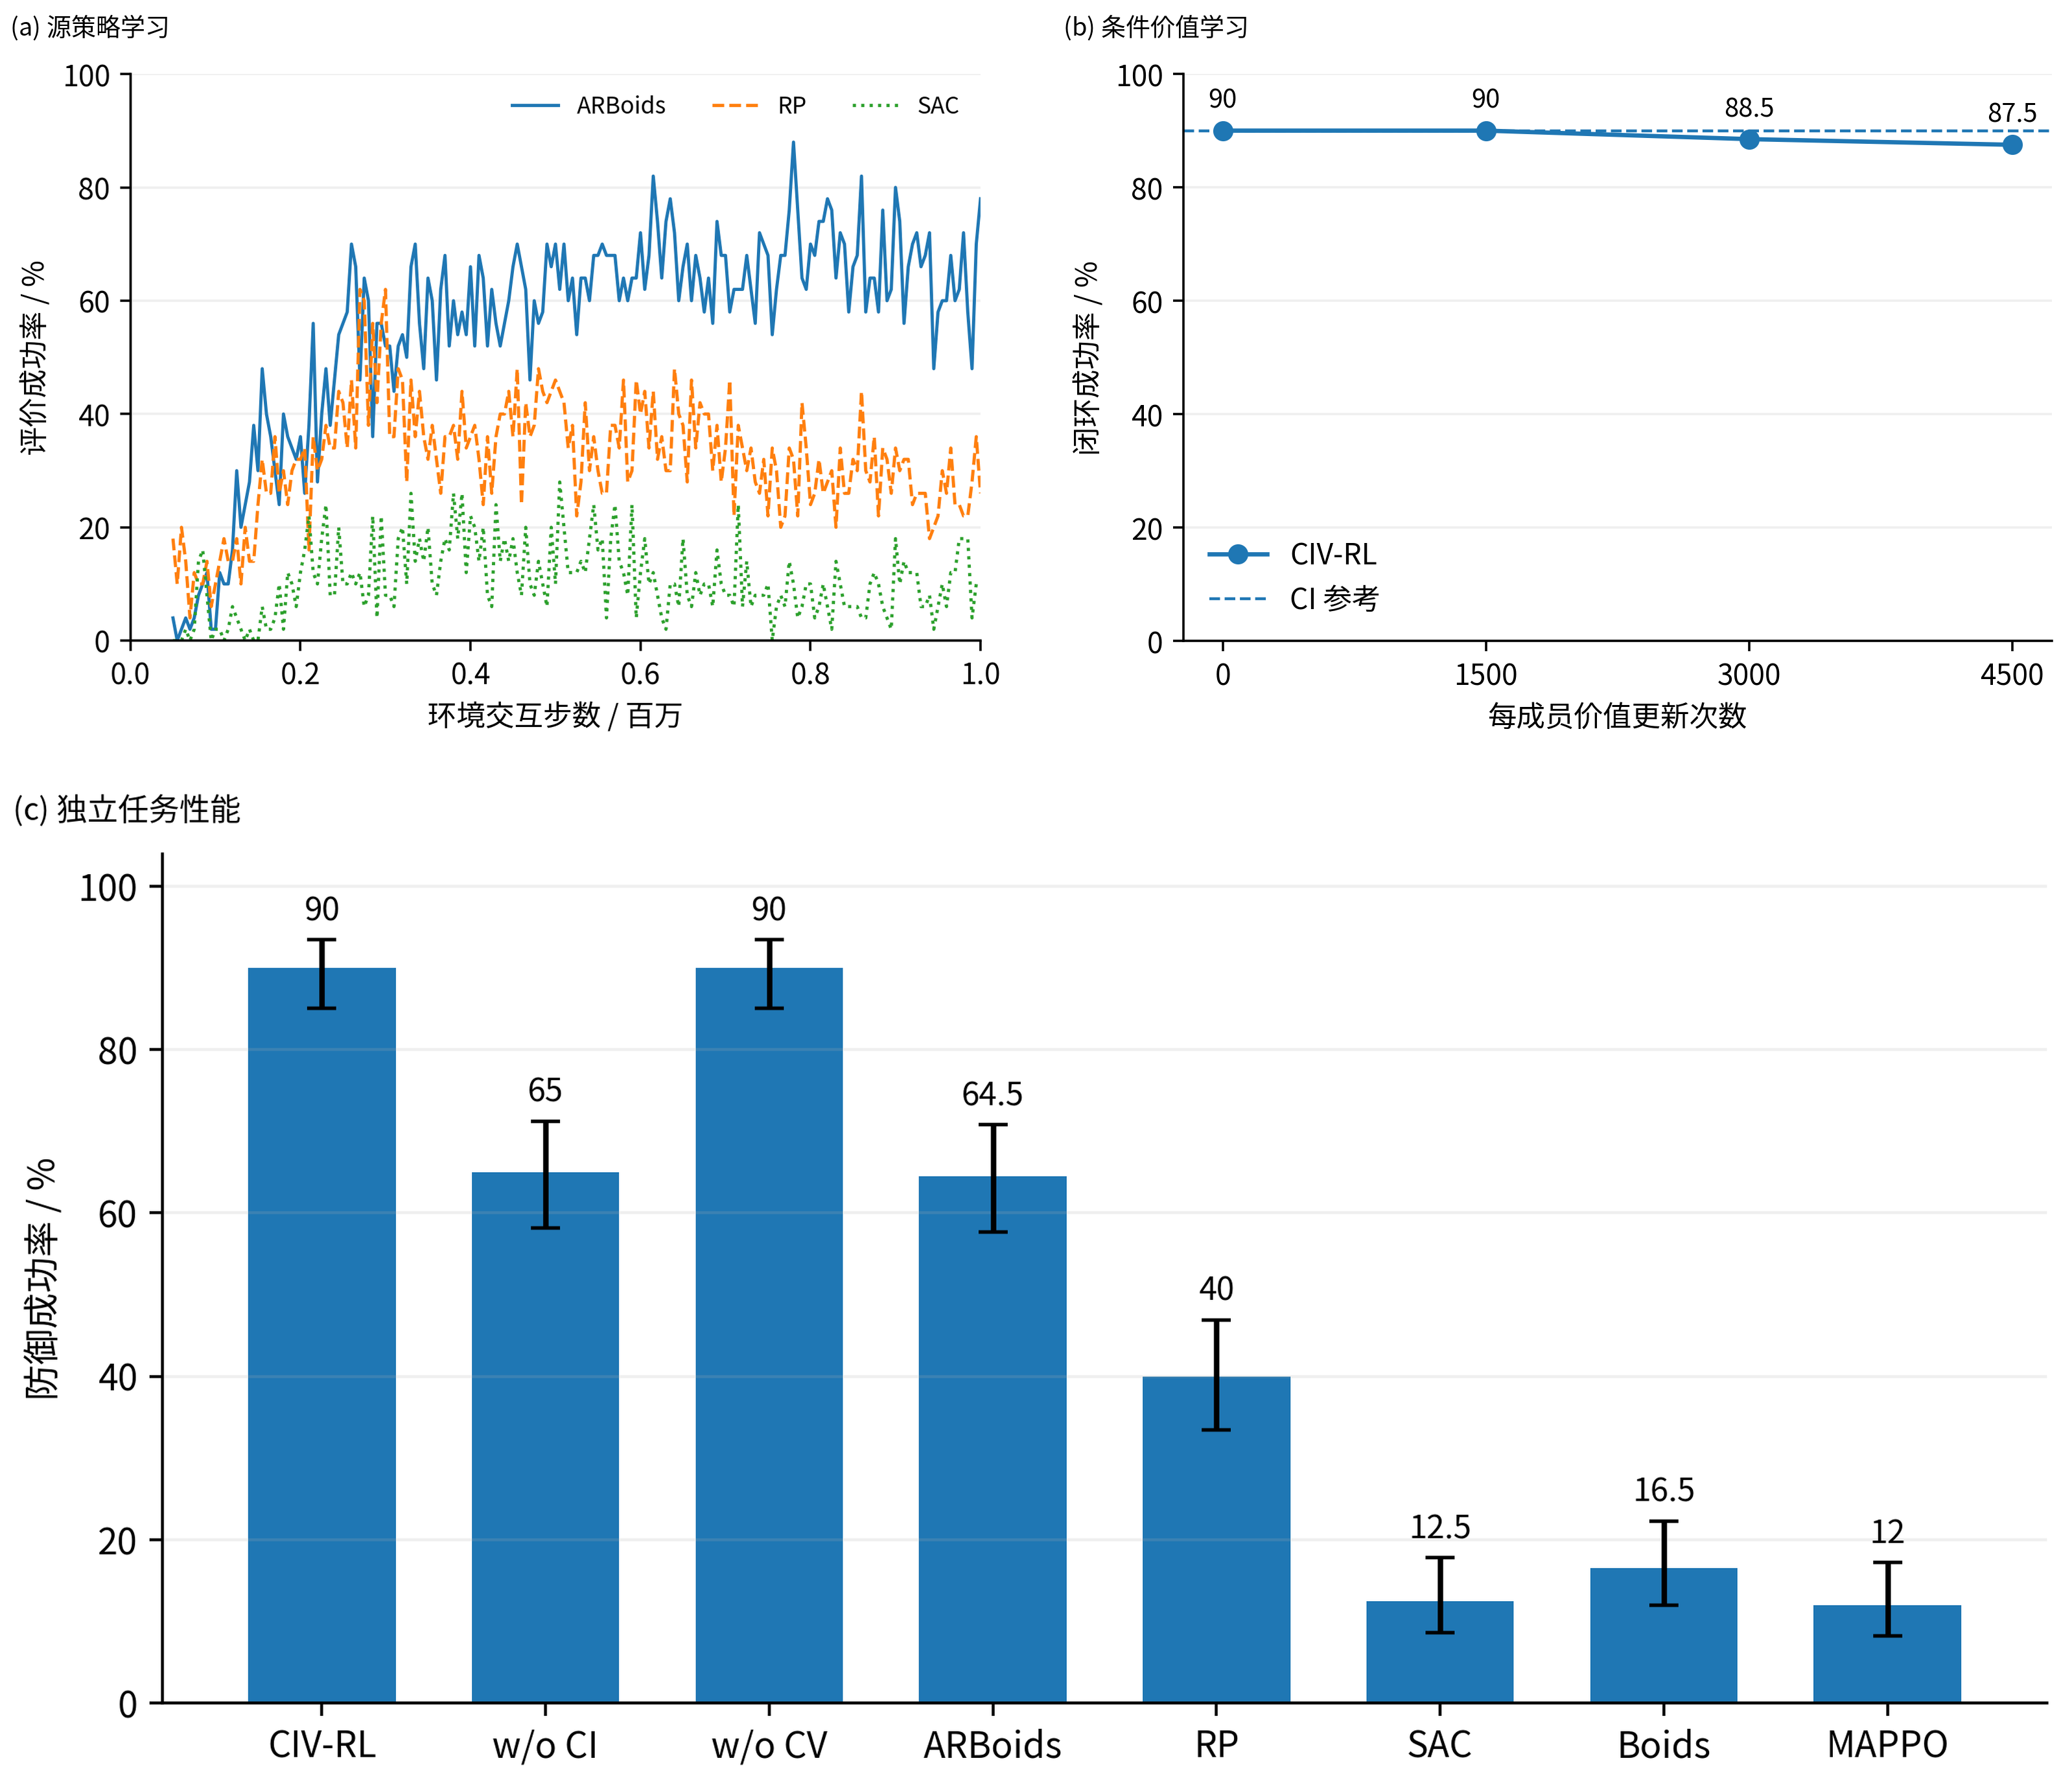
\includegraphics[width=6.35in]{figures/fig5_performance.png}
\caption{学习过程及独立任务性能。（a）源策略的实际训练评价记录，训练种子为42。（b）三个CV成员在相同更新进度下的完整闭环成功率，零次更新对应CI参考。（c）八种冻结方法在200个配对任务上的成功率，误差棒为任务比例的Wilson 95\%置信区间。}
\label{fig:5}
\end{figure}


在200个共同任务中，CIV-RL完成180次防御，成功率为90.0\%，95\%置信区间为85.06\%至93.43\%。ARBoids、RP、SAC、Boids和MAPPO的成功率分别为64.5\%、40.0\%、12.5\%、16.5\%和12.0\%。相对于ARBoids，完整方法增加51次成功，成功率提高25.5个百分点，艇间碰撞由70次减少至5次。相对于RP，成功率提高50.0个百分点，碰撞由115次减少至5次。CIV-RL的180次成功全部通过捕获完成，物理突破记录为零，任务失败由5次碰撞和15次径向失守组成。

\Needspace{6\baselineskip}
\begin{center}\small 表3　统一任务下的算法性能\end{center}

\begingroup\small
\begin{longtable}[]{@{}
  >{\raggedright\arraybackslash}p{(\columnwidth - 10\tabcolsep) * \real{0.1667}}
  >{\raggedright\arraybackslash}p{(\columnwidth - 10\tabcolsep) * \real{0.1667}}
  >{\raggedright\arraybackslash}p{(\columnwidth - 10\tabcolsep) * \real{0.1667}}
  >{\raggedright\arraybackslash}p{(\columnwidth - 10\tabcolsep) * \real{0.1667}}
  >{\raggedright\arraybackslash}p{(\columnwidth - 10\tabcolsep) * \real{0.1667}}
  >{\raggedright\arraybackslash}p{(\columnwidth - 10\tabcolsep) * \real{0.1667}}@{}}
\toprule\noalign{}
\begin{minipage}[b]{\linewidth}\raggedright
方法
\end{minipage} & \begin{minipage}[b]{\linewidth}\raggedright
成功率／\%
\end{minipage} & \begin{minipage}[b]{\linewidth}\raggedright
捕获率／\%
\end{minipage} & \begin{minipage}[b]{\linewidth}\raggedright
碰撞率／\%
\end{minipage} & \begin{minipage}[b]{\linewidth}\raggedright
物理突破率／\%
\end{minipage} & \begin{minipage}[b]{\linewidth}\raggedright
捕获时间／s
\end{minipage} \\
\midrule\noalign{}
\endhead
\bottomrule\noalign{}
\endlastfoot
CIV-RL & 90.0 & 90.0 & 2.5 & 0.0 & 24.02 \\
w/o CI & 65.0 & 65.0 & 34.0 & 0.0 & 18.78 \\
w/o CV & 90.0 & 90.0 & 2.5 & 0.0 & 24.84 \\
ARBoids & 64.5 & 64.5 & 35.0 & 0.0 & 18.86 \\
RP & 40.0 & 40.0 & 57.5 & 0.0 & 14.57 \\
SAC & 12.5 & 12.5 & 37.5 & 16.5 & 16.80 \\
Boids & 16.5 & 16.5 & 83.5 & 0.0 & 9.13 \\
MAPPO & 12.0 & 7.5 & 36.5 & 42.0 & 14.81 \\
\end{longtable}
\endgroup

w/o CI的成功率为65.0\%，完整方法较其增加50次成功。w/o
CV与完整方法同为90.0\%，两者的碰撞次数均为5次。由此，整体任务优势主要体现于候选运动的联合配置，而条件价值参与后维持了该组任务的防御水平。图5中源策略学习以环境交互步数表示，CV学习以各成员更新次数表示。CV在1
500、3 000和4
500次更新的冻结评价成功率分别为90.0\%、88.5\%和87.5\%，最终采用开发阶段选定的1
500次更新模型。该序列记录了同一控制基础上价值学习与实际闭环表现之间的对应。

\subsubsection{4.3.2
候选交互联合决策}\label{ux5019ux9009ux4ea4ux4e92ux8054ux5408ux51b3ux7b56}

联合与独立融合选择使用相同源策略、候选控制、局部评价和预测艇对代价。独立方法根据队友候选的局部偏好构造分布

\[
\rho_j(\ell\mid x)=
\frac{\exp[-\phi_j(\ell;x)]}
{\sum_{q=1}^{K_j}\exp[-\phi_j(q;x)]},
\tag{32}
\]

并由各艇分别选择期望代价最小的候选

\[
k_i^{\mathrm{ind}}\in\arg\min_k
\left[
\phi_i(k;x)+\lambda\sum_{j\ne i}
\sum_{\ell=1}^{K_j}\rho_j(\ell\mid x)\psi_{ij}(k,\ell;x)
\right].
\tag{33}
\]

两种选择器均读取艇对候选信息，分别通过联合配置能量和局部期望代价确定整队动作。在200个正式任务中，独立选择完成163次防御，CI完成180次，成功率由81.5\%提高至90.0\%。逐任务比较中，联合选择取得26次有利变化和9次不利变化，净增17次成功，对应8.5个百分点的增益，配对95\%区间为3.0至14.5个百分点。艇间碰撞由10次减至5次。该比较将候选运动信息保持一致，任务差异对应于对候选组合进行联合求解的作用。

当多个艇的局部偏好同时指向相互接近的运动时，式（13）以双方候选的组合代价协调融合系数。独立期望评价将队友的多种选择平均纳入局部得分，联合选择则评价实际共同执行的整组组合。成功率与碰撞次数的同步变化与这一决策依赖相联系，说明候选交互的作用需要在整队配置层面体现。表4汇总联合选择、条件价值及普通价值替代的直接比较。

\Needspace{12\baselineskip}
\begin{center}\small 表4　候选交互与条件价值的直接比较\end{center}

\begingroup\small
\begin{longtable}[]{@{}llllll@{}}
\toprule\noalign{}
配对比较 & 成功数 & 救回 & 损害 & 成功率差／百分点 & 95\%区间 \\
\midrule\noalign{}
\endhead
\bottomrule\noalign{}
\endlastfoot
CI相对独立选择 & 180／163 & 26 & 9 & 8.5 & {[}3.0, 14.5{]} \\
CIV-RL相对仅CI & 180／180 & 4 & 4 & 0.0 & {[}-3.0, 2.5{]} \\
CV相对普通价值 & 180／179 & 4 & 3 & 0.5 & {[}-2.0, 3.0{]} \\
\end{longtable}
\endgroup

\subsubsection{4.3.3
条件价值与融合选择}\label{ux6761ux4ef6ux4ef7ux503cux4e0eux878dux5408ux9009ux62e9}

条件价值与普通终局价值对照采用相同CI参考、根状态、联合候选和关系网络。普通模型以完整方案成功标签为监督，各输出共同拟合终局成功概率；条件模型采用式（24）至式（26）学习事实结果条件下的候选后果与配对收益。两种模型使用相同的候选接受接口及开发验证规则，选定的方案通过相同闭环过程执行。

完整CIV-RL在主评价中接受38次候选方案，相对于仅CI产生4次救回和4次损害，最终成功数均为180。普通价值方法完成179次成功，条件价值相对其产生4次救回与3次损害，净增1次成功。完整方法与仅CI共同捕获的176个任务中，配对捕获时间平均变化为\(-0.83\)
s。条件价值参与后的平均捕获回合耗时为24.02 s，仅CI为24.84
s，成功率保持90.0\%。该组结果表现为既有防御水平上的候选机动调整，终局数量和时间统计分别描述其任务完成与执行过程。

条件价值的直接辨识评价在未参与拟合的根状态上开展。以\(\mathcal P_{\ne}\)表示经验价值存在差异的候选对集合，排序一致率与收益误差为

\[
\begin{aligned}
A_{\mathrm{ord}}&=\frac{1}{|\mathcal P_{\ne}|}
\sum_{(x,z,z')\in\mathcal P_{\ne}}
\mathbb I\{\Delta_\theta(x;z,z')\widehat\Delta(x;z,z')>0\},\\
E_\Delta&=\mathbb E
\bigl[\Delta_\theta(x;z,z')-\widehat\Delta(x;z,z')\bigr]^2.
\end{aligned}
\tag{34}
\]

CV与普通价值模型的排序一致率分别为［　］和［　］，收益误差分别为［　］和［　］。相应候选辨识结果与表4的闭环配对结果共同刻画学习价值在融合选择中的作用。

\subsubsection{4.3.4 关键参数}\label{ux5173ux952eux53c2ux6570}

交互权重和候选接受阈值在100个开发任务中进行小规模分析。CI取\(\lambda\in\{0,16,32,64\}\)时，成功率分别为66.0\%、91.0\%、91.0\%和89.0\%，碰撞次数分别为34、2、3和4。引入艇对交互后，联合候选能够同时保持较高成功率和较低碰撞水平，名义权重附近的结果体现了交互项的有效作用区间。

固定价值网络与联合候选时，接受阈值\(\varepsilon\in\{0,0.025,0.075,0.15\}\)对应的成功率分别为95.0\%、95.0\%、95.0\%和92.0\%，候选接受次数分别为71、49、16和2。阈值为0.075时，相对于仅CI增加4次成功，配对结果为4次救回与零次损害。该组参数关系体现了接受门槛对候选执行频率及净结果的调节，完整数据列于补充表S1。正式主评价采用固定的\(\lambda=32\)与\(\varepsilon=0.075\)。

\subsection{4.4
攻击者机动性}\label{ux653bux51fbux8005ux673aux52a8ux6027}

机动性试验固定防御艇数为6，使用同一源策略、CI参数与条件价值模型，攻击者机动系数取1.0、1.5、2.0、2.5、3.0和3.5，各评价24个配对任务。图6(a)给出完整方法、仅CI、ARBoids及RP的成功率。各机动等级分别形成独立统计，初始几何与未来扰动在同一等级内保持配对。

CIV-RL在六个等级中分别完成22、22、19、23、23和15次防御，成功率为91.67\%、91.67\%、79.17\%、95.83\%、95.83\%和62.50\%。在\(L_{\mathrm{agi}}=2.5\)和3.0时，ARBoids分别完成18次和15次，RP分别完成13次和9次，而完整方法均完成23次且未发生艇间碰撞。在\(L_{\mathrm{agi}}=3.5\)时，完整方法与ARBoids均完成15次防御，碰撞次数分别为3次和9次。不同机动条件下的成功与碰撞统计共同体现了联合配置对艇间分离的持续作用。

\subsection{4.5
未见艇队规模}\label{ux672aux89c1ux8247ux961fux89c4ux6a21}

规模评价采用六艇训练完成的冻结源策略与条件价值模型，测试3、4、5、7和8艘防御艇，每个未见规模使用24个配对任务。六艇参考点由机动性2.0和2.5的48个任务组成。CI在当前艇集合上构造候选交互，CV通过共享节点映射及艇队聚合评价对应完整方案，各规模均使用相同融合参数和接受规则。图6(b)展示冻结策略在不同艇数下的任务表现。

\begin{figure}[htbp]
\centering
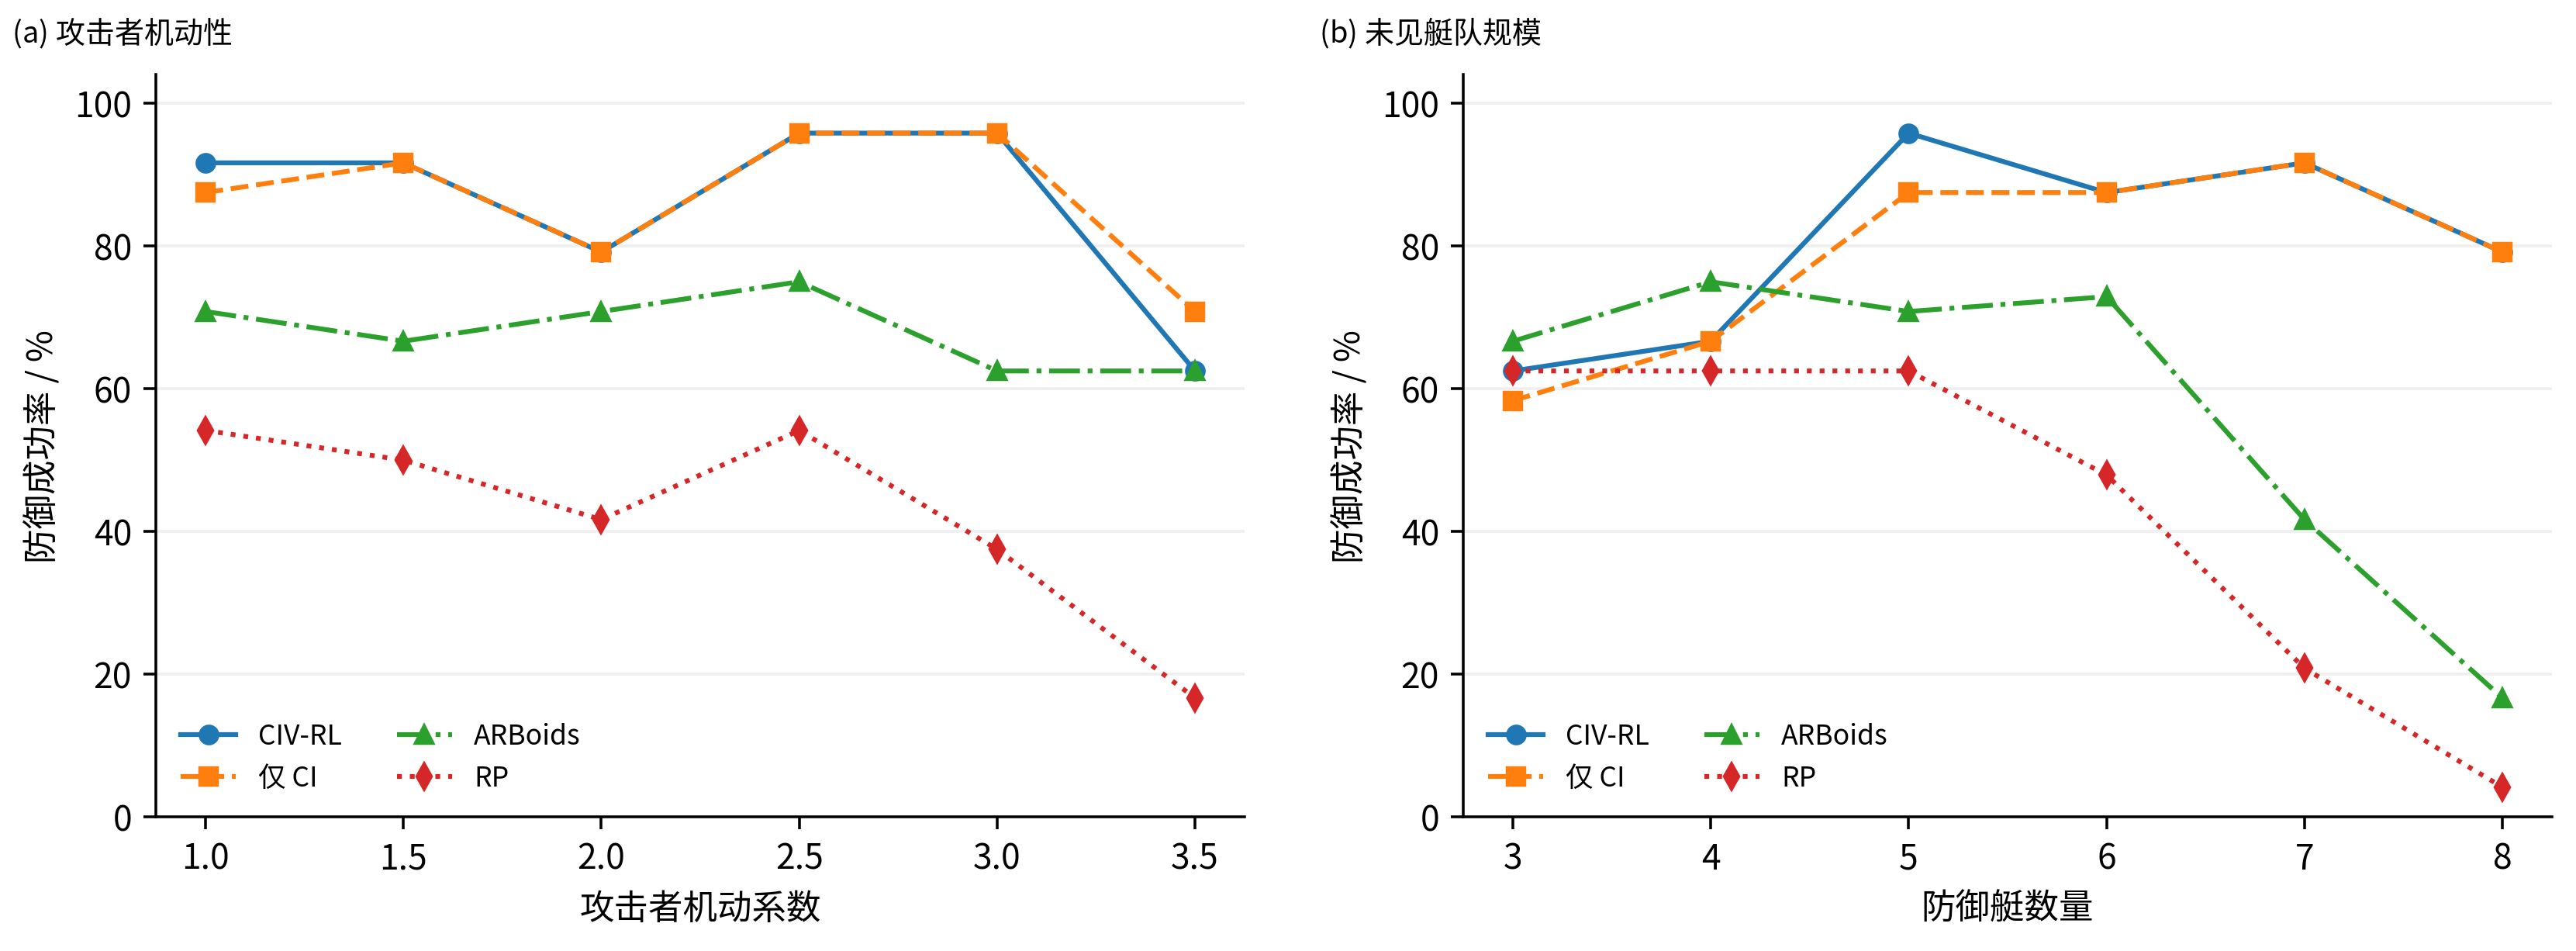
\includegraphics[width=6.35in]{figures/fig6_scope.png}
\caption{冻结策略的机动性与规模评价。（a）六艇条件下各机动等级使用24个任务。（b）各未见规模使用24个任务，六艇参考点使用48个任务。两组试验均采用相同冻结模型。}
\label{fig:6}
\end{figure}


在5、7和8艘艇条件下，CIV-RL分别完成23/24、22/24和19/24次防御，ARBoids分别完成17/24、10/24和4/24次。相应CIV-RL碰撞次数为0、0和4，ARBoids为5、14和20。较密集艇队中的性能差异与艇对候选的联合评价相对应，增加防御艇时，CI能够在多种局部融合组合中保持较好的运动相容性。

在3艘和4艘艇条件下，完整方法分别完成15/24和16/24次防御，ARBoids分别完成16/24和18/24次。相对于仅CI，完整方法在3艘和5艘艇条件下分别增加1次和2次成功，其余测试规模的成功数保持一致。各规模下候选价值仍由同一共享模型给出，联合融合与价值选择共同作用于当前艇队的控制组成。

\subsection{4.6
学习型攻击者}\label{ux5b66ux4e60ux578bux653bux51fbux8005}

对手适应试验首先冻结当前CIV-RL，使已训练的SAC攻击者继续与该防御策略交互，随后固定更新后的攻击者并继续学习条件价值模型。攻击阶段新增32
883步环境交互，在新增0、8 000、16 000及32
883步时使用相同64个任务评价。各阶段完整防御成功数分别为55、59、55和59，碰撞次数分别为1、1、0和0。图7(a)按照实际新增交互量记录这一过程，防御成功率处于85.94\%至92.19\%。

防御更新阶段从当前攻击策略下的192个任务中获得190个可行动根状态，每个根状态使用两组配对未来，共形成4
180条闭环分支。CI保持固定，条件价值网络根据新的对抗后果继续训练。另一个训练阶段将原人工势场任务的参考与候选观测共同纳入，形成兼顾当前对手与原任务的价值学习。图7(b)分别给出两类攻击条件下的结果。

\begin{figure}[htbp]
\centering
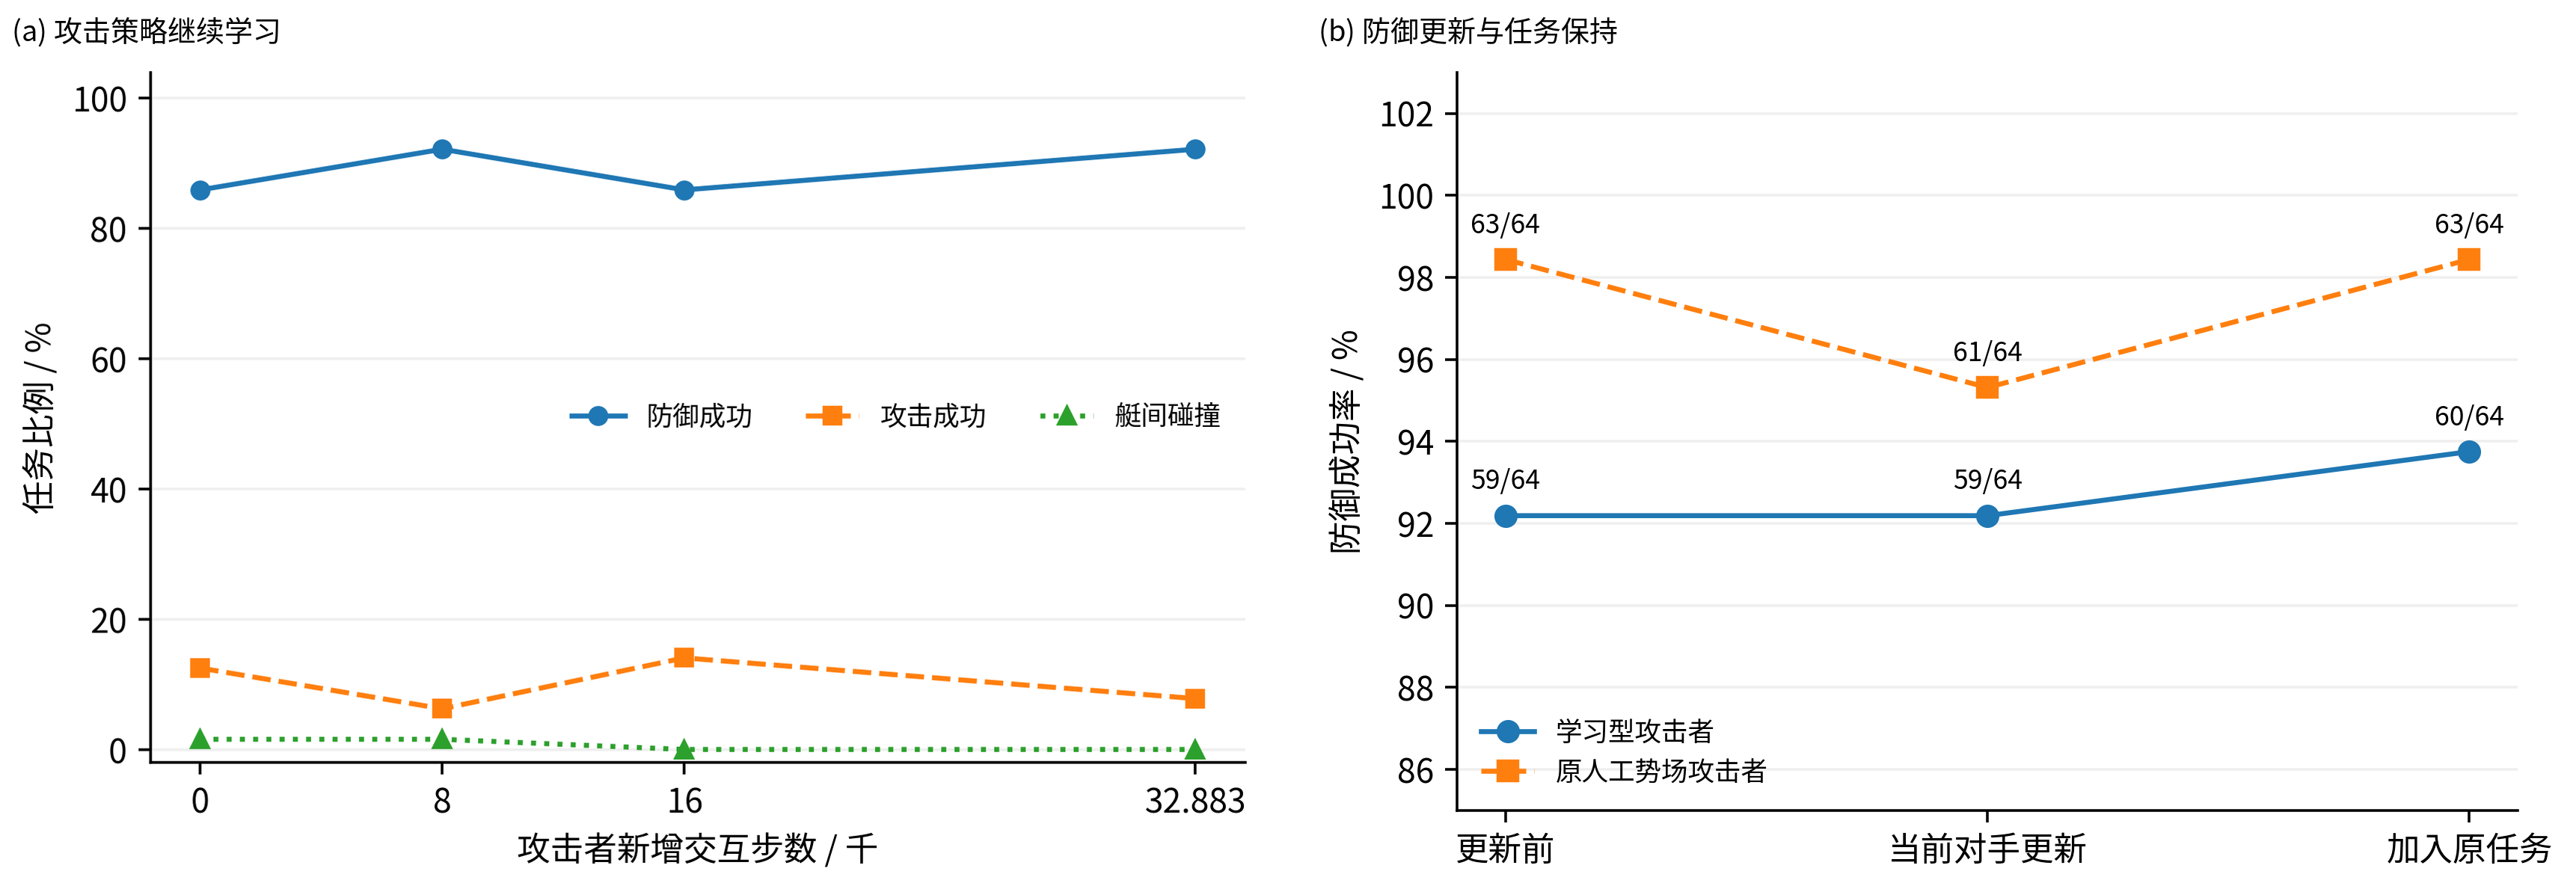
\includegraphics[width=6.35in]{figures/fig7_adaptation.png}
\caption{学习型攻击者与防御策略更新。（a）攻击者继续学习过程中的64任务评价。（b）防御更新前后在学习型攻击者和原人工势场攻击者下的任务表现，图中标注成功数。}
\label{fig:7}
\end{figure}


在最终学习型攻击者下，更新前、当前对手数据更新后以及加入原任务数据后，CIV-RL分别完成59/64、59/64和60/64次防御。原人工势场攻击者下的对应结果为63/64、61/64和63/64。加入原任务观测后的策略在两类对手下分别达到93.75\%和98.44\%的成功率，两组评价均未出现艇间碰撞。条件价值在固定联合融合结构中利用新的闭环结果更新候选评价，原任务与新对手数据共同参与时保持了相应的任务完成水平。

\FloatBarrier
\Needspace{8\baselineskip}
\section{5 结论}\label{ux7ed3ux8bba}

本文提出以候选交互联合融合为核心的多无人艇协同防御方法CIV-RL。该方法将双推进器的规则与学习控制组成表示为团队配置，利用反馈运动预测建立艇对交互势，并结合局部融合先验进行联合求解。配对闭环条件价值学习以相同候选空间中的完整方案为对象，将参考成功条件、候选终局结果和相对收益联系起来，学习所得价值参与最终融合选择。

六艇独立任务评价中，完整方法取得90.0\%的防御成功率，较ARBoids提高25.5个百分点，艇间碰撞率由35.0\%降至2.5\%。相同候选与预测条件下，CI较独立融合选择提高8.5个百分点，表明显式联合配置对协同运动具有实际作用。条件价值参与后保持了90.0\%的成功率，并在共同捕获任务上获得较短的平均捕获时间。12组VRX配对场景均完成捕获，冻结策略在5、7和8艘艇条件下分别取得95.83\%、91.67\%和79.17\%的成功率。上述结果体现了候选运动交互对多艇融合控制的主要贡献，以及条件任务价值与联合控制组成相联系的决策能力。

\section{参考文献}\label{ux53c2ux8003ux6587ux732e}
\begingroup\small\raggedright\setlength{\parskip}{3pt}

\noindent\hangindent=1.7em\hangafter=1 [1] Qiao Y, Yin J, Wang W, et al.~Survey of deep learning for
autonomous surface vehicles in marine environments. IEEE Transactions on
Intelligent Transportation Systems, 2023, 24(4), 3678-3701. DOI \nolinkurl{10.1109/TITS.2023.3235911}.

\noindent\hangindent=1.7em\hangafter=1 [2] Fu H, Liu H H T. Guarding a territory against an intelligent
intruder. Strategy design and experimental verification. IEEE/ASME
Transactions on Mechatronics, 2020, 25(4), 1765-1772. DOI \nolinkurl{10.1109/TMECH.2020.2996901}.

\noindent\hangindent=1.7em\hangafter=1 [3] Chen Y, Wu Y, Yang H, et al.~A distributed pipeline for
collaborative pursuit in the target guarding problem. IEEE Robotics and
Automation Letters, 2024, 9(3), 2064-2071. DOI \nolinkurl{10.1109/LRA.2024.3349977}.

\noindent\hangindent=1.7em\hangafter=1 [4] Yan R, Duan X, Zou R, et al.~Multiplayer homicidal chauffeur
reach-avoid games. A pursuit enclosure function approach. Automatica,
2024, 167, 111770. DOI \nolinkurl{10.1016/j.automatica.2024.111770}.

\noindent\hangindent=1.7em\hangafter=1 [5] Fang X, Wang C, Xie L, Chen J. Cooperative pursuit with
multi-pursuer and one faster free-moving evader. IEEE Transactions on
Cybernetics, 2022, 52(3), 1405-1414. DOI \nolinkurl{10.1109/TCYB.2019.2958548}.

\noindent\hangindent=1.7em\hangafter=1 [6] Guo X, Cui R, Yan W. Pursuit-evasion games of marine surface
vessels using neural network-based control. IEEE Transactions on
Systems, Man, and Cybernetics. Systems, 2025, 55(1), 18-27. DOI \nolinkurl{10.1109/TSMC.2023.3347044}.

\noindent\hangindent=1.7em\hangafter=1 [7] Reynolds C W. Flocks, herds and schools. A distributed
behavioral model. Computer Graphics, 1987, 21(4), 25-34. DOI \nolinkurl{10.1145/37402.37406}.

\noindent\hangindent=1.7em\hangafter=1 [8] de Souza C, Newbury R, Cosgun A, et al.~Decentralized
multi-agent pursuit using deep reinforcement learning. IEEE Robotics and
Automation Letters, 2021, 6(3), 4552-4559. DOI \nolinkurl{10.1109/LRA.2021.3068952}.

\noindent\hangindent=1.7em\hangafter=1 [9] 夏家伟，朱旭芳，张建强，罗亚松，刘忠.
基于多智能体强化学习的无人艇协同围捕方法.
控制与决策，2023，38(5)，1438-1447. DOI \nolinkurl{10.13195/j.kzyjc.2022.0564}.

\noindent\hangindent=1.7em\hangafter=1 [10] Xue S, Zhao N, Wang L, et al.~Multi-agent self-attention
reinforcement learning for multi-USV hunting target. Neural Networks,
2025, 189, 107574. DOI \nolinkurl{10.1016/j.neunet.2025.107574}.

\noindent\hangindent=1.7em\hangafter=1 [11] Yu J, et al.~A cooperative hunting method for multi-USVs based
on trajectory prediction by OR-LSTM. IEEE Transactions on Vehicular
Technology, 2024, 73(12), 18087-18101. DOI \nolinkurl{10.1109/TVT.2024.3432739}.

\noindent\hangindent=1.7em\hangafter=1 [12] Hüttenrauch M, Šošić A, Neumann G. Deep reinforcement learning
for swarm systems. Journal of Machine Learning Research, 2019, 20(54),
1-31.

\noindent\hangindent=1.7em\hangafter=1 [13] Rashid T, Samvelyan M, de Witt C S, et al.~Monotonic value
function factorisation for deep multi-agent reinforcement learning.
Journal of Machine Learning Research, 2020, 21(178), 1-51.

\noindent\hangindent=1.7em\hangafter=1 [14] Yu C, Velu A, Vinitsky E, et al.~The surprising effectiveness
of PPO in cooperative multi-agent games. Advances in Neural Information
Processing Systems, 2022, 35, 24611-24624.

\noindent\hangindent=1.7em\hangafter=1 [15] Boehmer W, Kurin V, Whiteson S. Deep coordination graphs.
Proceedings of the 37th International Conference on Machine Learning,
2020, 119, 980-991.

\noindent\hangindent=1.7em\hangafter=1 [16] Ma Z, Luo Y, Pan J. Learning selective communication for
multi-agent path finding. IEEE Robotics and Automation Letters, 2022,
7(2), 1455-1462. DOI \nolinkurl{10.1109/LRA.2021.3139145}.

\noindent\hangindent=1.7em\hangafter=1 [17] Li Q, Lin W, Liu Z, Prorok A. Message-aware graph attention
networks for large-scale multi-robot path planning. IEEE Robotics and
Automation Letters, 2021, 6(3), 5533-5540. DOI \nolinkurl{10.1109/LRA.2021.3077863}.

\noindent\hangindent=1.7em\hangafter=1 [18] Johannink T, Bahl S, Nair A, et al.~Residual reinforcement
learning for robot control. Proceedings of the IEEE International
Conference on Robotics and Automation, 2019, 6023-6029. DOI \nolinkurl{10.1109/ICRA.2019.8794127}.

\noindent\hangindent=1.7em\hangafter=1 [19] Rana K, et al.~Bayesian controller fusion. Leveraging control
priors in deep reinforcement learning for robotics. The International
Journal of Robotics Research, 2023, 42(3), 123-146. DOI \nolinkurl{10.1177/02783649231167210}.

\noindent\hangindent=1.7em\hangafter=1 [20] Jeon S H, Lee H J, Hong S, Kim S. Residual MPC. Blending
reinforcement learning with GPU-parallelized model predictive control.
arXiv, 2025, 2510.12717.

\noindent\hangindent=1.7em\hangafter=1 [21] Tao J, Shen T, Zhao D, Zhang F. ARBoids. Adaptive residual
reinforcement learning with Boids model for cooperative multi-USV target
defense. IEEE Robotics and Automation Letters, 2026, 11(3), 3637-3644.
DOI \nolinkurl{10.1109/LRA.2026.3662620}.

\noindent\hangindent=1.7em\hangafter=1 [22] Foerster J, Farquhar G, Afouras T, et al.~Counterfactual
multi-agent policy gradients. Proceedings of the AAAI Conference on
Artificial Intelligence, 2018, 32(1), 2974-2982. DOI \nolinkurl{10.1609/aaai.v32i1.11794}.

\noindent\hangindent=1.7em\hangafter=1 [23] Bhattacharya S, Kailas S, Badyal S, Gil S, Bertsekas D.
Multiagent reinforcement learning. Rollout and policy iteration for
POMDP with application to multirobot problems. IEEE Transactions on
Robotics, 2024, 40, 2003-2023. DOI \nolinkurl{10.1109/TRO.2023.3347128}.

\noindent\hangindent=1.7em\hangafter=1 [24] Feinberg V, Wan A, Stoica I, Jordan M I, Gonzalez J E, Levine
S. Model-based value estimation for efficient model-free reinforcement
learning. arXiv, 2018, 1803.00101.

\noindent\hangindent=1.7em\hangafter=1 [25] Fossen T I. Handbook of Marine Craft Hydrodynamics and Motion
Control. Chichester, Wiley, 2011.

\noindent\hangindent=1.7em\hangafter=1 [26] Bingham B, Aguero C, McCarrin M, et al.~Toward maritime robotic
simulation in Gazebo. Proceedings of the MTS/IEEE OCEANS Conference,
2019, 1-10. DOI \nolinkurl{10.23919/OCEANS40490.2019.8962725}.

\noindent\hangindent=1.7em\hangafter=1 [27] Haarnoja T, Zhou A, Abbeel P, Levine S. Soft actor-critic.
Off-policy maximum entropy deep reinforcement learning with a stochastic
actor. Proceedings of the 35th International Conference on Machine
Learning, 2018, 80, 1861-1870.

\noindent\hangindent=1.7em\hangafter=1 [28] Bengio Y, Louradour J, Collobert R, Weston J. Curriculum
learning. Proceedings of the 26th Annual International Conference on
Machine Learning, 2009, 41-48. DOI \nolinkurl{10.1145/1553374.1553380}.

\endgroup
\clearpage
\section{补充材料}\label{ux8865ux5145ux6750ux6599}

\subsection{S1
关键参数敏感性}\label{s1-ux5173ux952eux53c2ux6570ux654fux611fux6027}

交互权重分析固定源策略、候选集合与预测时域，在同一开发任务中改变艇对代价的权重。接受阈值分析固定CI与CV模型，在相同任务中改变候选的价值接受门槛。两项结果分别反映运动交互与条件价值选择对闭环行为的作用，统计见表S1。

\Needspace{6\baselineskip}
\begin{center}\small 表S1　关键参数与配对任务结果\end{center}

\begingroup\small
\begin{longtable}[]{@{}
  >{\raggedright\arraybackslash}p{(\columnwidth - 14\tabcolsep) * \real{0.1250}}
  >{\raggedright\arraybackslash}p{(\columnwidth - 14\tabcolsep) * \real{0.1250}}
  >{\raggedright\arraybackslash}p{(\columnwidth - 14\tabcolsep) * \real{0.1250}}
  >{\raggedright\arraybackslash}p{(\columnwidth - 14\tabcolsep) * \real{0.1250}}
  >{\raggedright\arraybackslash}p{(\columnwidth - 14\tabcolsep) * \real{0.1250}}
  >{\raggedright\arraybackslash}p{(\columnwidth - 14\tabcolsep) * \real{0.1250}}
  >{\raggedright\arraybackslash}p{(\columnwidth - 14\tabcolsep) * \real{0.1250}}
  >{\raggedright\arraybackslash}p{(\columnwidth - 14\tabcolsep) * \real{0.1250}}@{}}
\toprule\noalign{}
\begin{minipage}[b]{\linewidth}\raggedright
参数
\end{minipage} & \begin{minipage}[b]{\linewidth}\raggedright
取值
\end{minipage} & \begin{minipage}[b]{\linewidth}\raggedright
成功率／\%
\end{minipage} & \begin{minipage}[b]{\linewidth}\raggedright
碰撞数
\end{minipage} & \begin{minipage}[b]{\linewidth}\raggedright
接受数
\end{minipage} & \begin{minipage}[b]{\linewidth}\raggedright
救回
\end{minipage} & \begin{minipage}[b]{\linewidth}\raggedright
损害
\end{minipage} & \begin{minipage}[b]{\linewidth}\raggedright
净增／百分点
\end{minipage} \\
\midrule\noalign{}
\endhead
\bottomrule\noalign{}
\endlastfoot
\(\lambda/\lambda_0\) & 0.0 & 66.0 & 34 & 0 & 4 & 29 & -25.0 \\
\(\lambda/\lambda_0\) & 0.5 & 91.0 & 2 & 0 & 6 & 6 & 0.0 \\
\(\lambda/\lambda_0\) & 1.0 & 91.0 & 3 & 0 & 0 & 0 & 0.0 \\
\(\lambda/\lambda_0\) & 2.0 & 89.0 & 4 & 0 & 4 & 6 & -2.0 \\
\(\varepsilon\) & 0.0 & 95.0 & 3 & 71 & 6 & 2 & 4.0 \\
\(\varepsilon\) & 0.025 & 95.0 & 3 & 49 & 6 & 2 & 4.0 \\
\(\varepsilon\) & 0.075 & 95.0 & 3 & 16 & 4 & 0 & 4.0 \\
\(\varepsilon\) & 0.15 & 92.0 & 3 & 2 & 1 & 0 & 1.0 \\
\end{longtable}
\endgroup

\subsection{S2
独立完整训练统计}\label{s2-ux72ecux7acbux5b8cux6574ux8badux7ec3ux7edfux8ba1}

独立完整训练以源策略、候选交互模型及其对应条件价值学习为共同运行单元。各运行采用相同训练配置与正式任务分布，源策略和价值学习使用各自独立随机初始化，统计结果按训练运行汇总。

\begingroup\small
\begin{longtable}[]{@{}
  >{\raggedright\arraybackslash}p{(\columnwidth - 14\tabcolsep) * \real{0.1250}}
  >{\raggedright\arraybackslash}p{(\columnwidth - 14\tabcolsep) * \real{0.1250}}
  >{\raggedright\arraybackslash}p{(\columnwidth - 14\tabcolsep) * \real{0.1250}}
  >{\raggedright\arraybackslash}p{(\columnwidth - 14\tabcolsep) * \real{0.1250}}
  >{\raggedright\arraybackslash}p{(\columnwidth - 14\tabcolsep) * \real{0.1250}}
  >{\raggedright\arraybackslash}p{(\columnwidth - 14\tabcolsep) * \real{0.1250}}
  >{\raggedright\arraybackslash}p{(\columnwidth - 14\tabcolsep) * \real{0.1250}}
  >{\raggedright\arraybackslash}p{(\columnwidth - 14\tabcolsep) * \real{0.1250}}@{}}
\toprule\noalign{}
\begin{minipage}[b]{\linewidth}\raggedright
统计量
\end{minipage} & \begin{minipage}[b]{\linewidth}\raggedright
CIV-RL
\end{minipage} & \begin{minipage}[b]{\linewidth}\raggedright
w/o CI
\end{minipage} & \begin{minipage}[b]{\linewidth}\raggedright
w/o CV
\end{minipage} & \begin{minipage}[b]{\linewidth}\raggedright
ARBoids
\end{minipage} & \begin{minipage}[b]{\linewidth}\raggedright
RP
\end{minipage} & \begin{minipage}[b]{\linewidth}\raggedright
SAC
\end{minipage} & \begin{minipage}[b]{\linewidth}\raggedright
MAPPO
\end{minipage} \\
\midrule\noalign{}
\endhead
\bottomrule\noalign{}
\endlastfoot
完整训练运行数 & ［　］ & ［　］ & ［　］ & ［　］ & ［　］ & ［　］ &
［　］ \\
防御成功率均值 & ［　］ & ［　］ & ［　］ & ［　］ & ［　］ & ［　］ &
［　］ \\
运行间标准差 & ［　］ & ［　］ & ［　］ & ［　］ & ［　］ & ［　］ &
［　］ \\
相对既定参考的平均配对差 & ［　］ & ［　］ & ［　］ & ［　］ & ［　］ &
［　］ & ［　］ \\
\end{longtable}
\endgroup

\end{document}
